\documentclass[lettersize,journal]{IEEEtran}
\IEEEoverridecommandlockouts
% \usepackage[utf8]{inputenc}

\usepackage{cite}
\usepackage[utf8x]{inputenc} 
\usepackage{amsmath,amssymb,amsfonts}
\usepackage{algorithmic}
\usepackage[table,xcdraw]{xcolor}
\usepackage{float}
\usepackage{graphicx}
\usepackage[shortlabels,inline]{enumitem}
\usepackage{makecell}
%\usepackage[style=base]{caption}
\usepackage{subcaption}
\usepackage{hyperref}
\usepackage{longtable}
\usepackage{multirow}
\usepackage{url}
\usepackage{pifont}
\usepackage{textcomp}
\usepackage{ragged2e}
\usepackage[linesnumbered,ruled,vlined]{algorithm2e}
\usepackage{bm}
\usepackage{arydshln}
\usepackage{caption}
\usepackage{multirow}
\usepackage{tabularray}
\usepackage{float}
\usepackage{colortbl}
\usepackage{orcidlink}
\usepackage{booktabs}
\usepackage{pgfplots}

\pgfplotsset{compat=1.16}
\usepackage{siunitx}
\usepackage{hhline}
\usepackage[font=footnotesize,labelfont=bf,
   justification=justified,
   format=plain,skip=0pt,belowskip=0pt,aboveskip=0pt]{caption}
\usepackage{textcomp}
\usepackage[normalem]{ulem}
\usepackage{tikz}

\usepackage[capitalise,nameinlink]{cleveref}
% \usepackage{color}
\usepackage[normalem]{ulem}
\usepackage{tabularray}
\UseTblrLibrary{diagbox}

\usepackage{etoolbox}

\newcommand{\zcolor}[1]{\textcolor{violet}{#1}}
\newcommand{\Acolor}[1]{\textcolor{black}{#1}}
\newcommand{\Jcolor}[1]{\textcolor{orange}{#1}}
\setlength{\intextsep}{0.3cm}
\setlength{\textfloatsep}{0.2cm}
\setlength{\floatsep}{0cm}
\SetAlgoSkip{}
\def\BibTeX{{\rm B\kern-.05em{\sc i\kern-.025em b}\kern-.08em
    T\kern-.1667em\lower.7ex\hbox{E}\kern-.125emX}}

\newcommand*\circled[1]{\tikz[baseline=(char.base)]{
            \node[shape=circle,draw,inner sep=2pt] (char) {#1};}}

\newcommand{\cmark}{\textcolor{green!50!black}{\ding{51}}}%
\newcommand{\xmark}{\textcolor{red}{\ding{55}}}%
%\newcommand{\SYS}{QUEST}
\newcommand{\SYS}[0]{{{QUEST}}\xspace}

\markboth{IEEE Internet of Things,~Vol.~x, No.~x, April.~2025}%
{Younesi \MakeLowercase{\textit{et al.}}: \textit{FLARE}: Adaptive Multi-Dimensional Reputation for Robust Client Reliability in Federated Learning}
\begin{document}

% \newtheorem{theorem}{Theorem}
% \newtheorem*{proofsketch}{Proof (Sketch)}

\title{\textit{FLARE}: Adaptive Multi-Dimensional Reputation for Robust Client Reliability in Federated Learning}

\author{Abolfazl Younesi\IEEEauthorrefmark{1}\,\orcidlink{0009-0003-0052-6475}\,(\IEEEmembership{Student, IEEE}),
Leon Kiss\IEEEauthorrefmark{1}\,\orcidlink{0009-0003-7103-6430},
Zahra Najafabadi Samani\IEEEauthorrefmark{1}\,\orcidlink{0000-0001-5182-9087},
Juan Aznar Poveda\IEEEauthorrefmark{1}\,\orcidlink{0000-0002-0879-6651}\,
Thomas Fahringer\IEEEauthorrefmark{1}\,\orcidlink{0000-0003-4293-1228}\,(\IEEEmembership{Member, IEEE})
        % <-this % stops a space
\thanks{Manuscript received XX May. 2025; revised XX Aug. 2025 and xx yy 202x; accepted xx yy 202x. Date of publication xx yy 202x; date of current version x June 202x. (Corresponding author: Abolfazl Younesi.)

A. Younesi, L. Kiss, Z. N. Samani, J. A. Poveda, and T. Fahringer are with the Department of Computer Science, University of Innsbruck, Innsbruck, Austria. E-mails: \{Abolfazl.Younesi, Leon.Kiss, Zahra.Najafabadi-Samani, Juan.Aznar-Poveda, Thomas.Fahringer\}@uibk.ac.at
}}


\maketitle



\begin{abstract}
Federated learning (FL) enables collaborative model training while preserving data privacy. However, it remains vulnerable to malicious clients who compromise model integrity through Byzantine attacks, data poisoning, or adaptive adversarial behaviors. Existing defense mechanisms rely on static thresholds and binary classification, failing to adapt to evolving client behaviors in real-world deployments. We propose \textit{FLARE}, an adaptive reputation-based framework that transforms client reliability assessment from binary decisions to a continuous, multi-dimensional trust evaluation. 
FLARE integrates: \textbf{(i)} a multi-dimensional reputation score capturing performance consistency, statistical anomaly indicators, and temporal behavior, \textbf{(ii)} a self-calibrating adaptive threshold mechanism that adjusts security strictness based on model convergence and recent attack intensity, \textbf{(iii)} reputation-weighted aggregation with soft exclusion to proportionally limit suspicious contributions rather than eliminating clients outright, and \textbf{(iv)} a Local Differential Privacy (LDP) mechanism enabling reputation scoring on privatized client updates.
We further introduce a highly evasive \emph{Statistical Mimicry (SM)} attack, a benchmark adversary that blends honest gradients with synthetic perturbations and persistent drift to remain undetected by traditional filters. Extensive experiments with 100 clients on MNIST, CIFAR-10, and SVHN demonstrate that \textit{FLARE} maintains high model accuracy and converges faster than state-of-the-art Byzantine-robust methods under diverse attack types, including label flipping, gradient scaling, adaptive attacks, ALIE, and SM. FLARE improves robustness by up to 16\% and preserves model convergence within 30\% of the non-attacked baseline, while achieving strong malicious-client detection performance with minimal computational overhead.
\url{https://github.com/Anonymous0-0paper/FLARE}
\end{abstract}


% \begin{abstract}
% Federated learning (FL) enables collaborative model training while preserving data privacy. However, it remains vulnerable to malicious clients who compromise model integrity through Byzantine attacks, data poisoning, or adaptive adversarial behaviors. Existing defense mechanisms rely on static thresholds and binary classification, failing to adapt to evolving client behaviors in real-world deployments. We propose \textit{FLARE}, a reputation-based framework that transforms client reliability assessment from a binary classification to a continuous, multi-dimensional trust evaluation. Our framework integrates: \textbf{(i)} a multi-dimensional reputation score evaluating clients across performance, statistical, and temporal dimensions, \textbf{(ii)} an adaptive threshold mechanism that adjusts security posture based on model convergence, \textbf{(iii)} reputation-weighted aggregation with soft exclusion, and \textbf{(iii)} a Local Differential Privacy (LDP) model that enables scoring on client-privatized data. We validate our framework against multiple threats, including a highly evasive Statistical Mimicry (SM) attack, which we introduce as a challenging benchmark for stealthy, cumulative-drift adversaries. Extensive experiments with 100 clients across the MNIST, CIFAR-10, and SVHN datasets demonstrate that \textit{FLARE} maintains high model accuracy and converges faster than Byzantine-robust methods under various standard attacks, providing a clear benchmark for its defensive capabilities.
% \end{abstract}

\begin{IEEEkeywords}
Federated learning, Reputation, Byzantine attacks, Client, Reliability, Trust management, Robust aggregation
\end{IEEEkeywords}

\section{Introduction}
%-------------------------------------------------------------------------------

Federated learning (FL) has emerged as a pivotal paradigm for training machine learning models across distributed devices while preserving data privacy \cite{guo2025reputation,shi2025fedmar,8832210,YOUNESI2026101815}. By enabling collaborative model training without centralizing raw data, FL addresses critical privacy concerns in domains ranging from healthcare to financial services. Participating clients in FL, such as smartphones, wearable devices, or edge servers, locally compute model updates using their private data and send only the updated parameters to a central server, which aggregates them into a global model \cite{pmlr-v54-mcmahan17a}. This decentralized approach not only minimizes data exposure but also reduces the burden of data transfer and storage, making FL particularly suitable for large-scale, privacy-sensitive applications. The promise of FL lies in its ability to harness the collective intelligence of numerous devices while respecting individual privacy \cite{li2020federated,kairouz2021advancesopenproblemsfederated,younesi2024cnn}.
Despite its advantages, the distributed and open nature of FL introduces security and trust challenges. Unlike traditional centralized training, where the data and computation are under the control of a single trusted entity, FL operates in a loosely coordinated environment where clients are autonomous and often unverified \cite{lyu2020threats,bagdasaryan2020backdoor}. This autonomy creates opportunities for malicious or unreliable participants to inject harmful updates, skew the global model, or exploit the system for personal gain. The lack of direct oversight, combined with the diversity of hardware, network conditions, and user behaviors, further complicates the task of ensuring consistent and trustworthy collaboration.
\Acolor{As an illustrative example,} Figure~\ref{fig:motivation} demonstrates how traditional static approaches to client reliability assessment can suffer from critical misclassification errors: they may permanently exclude honest clients experiencing transient network issues or possessing unique data distributions, while failing to detect sophisticated adaptive attackers who manipulate their behavior to evade detection. As FL deployments scale across thousands of geographically dispersed devices with varying trustworthiness, the need for robust, adaptive mechanisms to assess and manage client reliability becomes increasingly urgent.

% added by thomas
Beyond adversarial behavior, unreliable client participation may also arise from intermittent connectivity, volatile execution environments, or heterogeneous device capabilities. Such instability has been widely observed in distributed computing environments, cloud platforms, and intelligent edge systems, where node reliability cannot be assumed to remain static over time and may fluctuate unpredictably under workload pressure or resource constraints. This observation is consistent with prior studies showing that dynamic availability and behavioral variability affect the stability of large-scale distributed and cloud systems, necessitating adaptive mechanisms rather than fixed trust assumptions \cite{8457785,9090348}.

\begin{figure*}
    \centering
    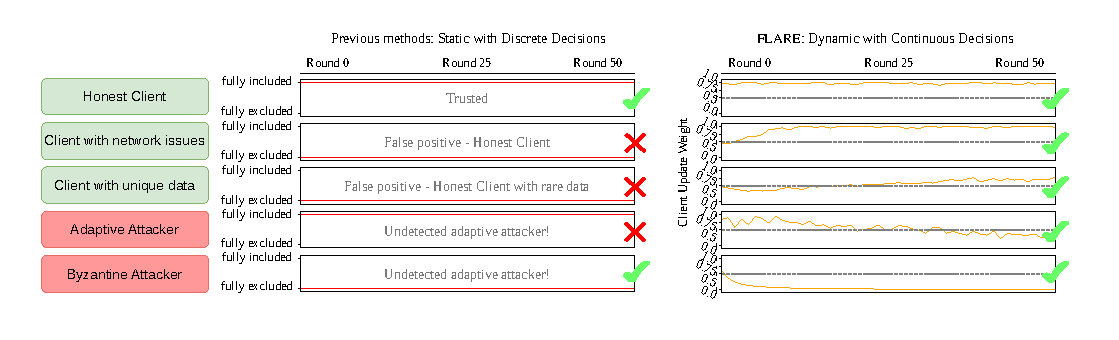
\includegraphics[width=1\linewidth]{framework-comparison.pdf}
    \caption{Comparison of client reliability assessment approaches in federated learning. \textbf{Left:} Previous static methods make binary inclusion/exclusion decisions that remain fixed throughout training, leading to false positives for honest clients with temporary issues or unique data distributions, while failing to detect adaptive attackers. \textbf{Right:} Our \textit{FLARE} framework uses dynamic reputation scoring with continuous weight adjustments, enabling nuanced trust assessments that adapt to evolving client behavior over time. }
    \label{fig:motivation}
\end{figure*}
% However, this distributed nature introduces a fundamental vulnerability: the presence of unreliable or malicious clients that can compromise model integrity through Byzantine attacks, data poisoning, or free-riding behaviors \cite{zhao2022deepleakagemodelfederated}. As illustrated in Figure~\ref{fig:motivation}, traditional static approaches suffer from critical misclassification errors. They permanently exclude honest clients experiencing temporary network issues or possessing unique data distributions, while simultaneously failing to detect sophisticated adaptive attackers who strategically manipulate their behavior to evade detection.

\textbf{Challenges.} The challenge of identifying and mitigating unreliable clients in FL systems remains particularly acute due to three inherent characteristics of federated environments. First, the heterogeneity of client devices and data distributions makes it difficult to distinguish between legitimate statistical variations and adversarial behaviors \cite{le2025byzantineresilientfederatedmultitask,liu2022decentralized}. Second, the privacy-preserving nature of FL limits the server's visibility into client operations, creating an information asymmetry that malicious actors can exploit \cite{chen2024federated,kumar2023impact}. Third, the dynamic nature of real-world FL deployments, where clients may join, leave, or change their behavior patterns over time, renders static detection mechanisms ineffective \cite{chen2024federated,el2021distributed,farhadkhani2022byzantine}.


\textbf{Existing approaches.} Existing approaches to client reliability assessment in FL primarily fall into two categories: Byzantine-robust aggregation methods and client selection strategies \cite{yin2018byzantine,el2021distributed,farhadkhani2022byzantine,10147260,blanchard2017machine}. Byzantine-robust aggregation techniques, such as Krum~\cite{blanchard2017machine} and trimmed mean~\cite{yin2018byzantine}, attempt to minimize the impact of malicious updates through statistical filtering. While these methods provide theoretical guarantees under specific attack models, they often struggle with adaptive adversaries and can inadvertently exclude benign clients with unique data distributions. Client selection strategies, on the other hand, aim to identify trustworthy participants preemptively based on their historical performance or validation accuracy~\cite{fang2024byzantine,zhao2022fedinv,10713463}. 

\textbf{Limitations.} The existing approaches employ static thresholds and binary classification schemes that fail to capture the nuanced and evolving nature of client reliability. These limitations become particularly pronounced in dynamic FL environments where client behaviors evolve over time \cite{11082298,zhao2020local,fang2024byzantine,zhao2022fedinv,penalva2025repunet,tan2022reputation,al2023reputation,fu2022label}. A client that initially appears reliable may become compromised or experience performance degradation, while suspicious clients may prove trustworthy as more information becomes available. 

Furthermore, sophisticated adversaries can strategically manipulate their behavior to evade detection, alternating between benign and malicious actions to maintain acceptable aggregate metrics while still degrading model performance. 
Existing methods also suffer from three critical shortcomings \cite{zhao2020local,fang2024byzantine,zhao2022fedinv,penalva2025repunet,tan2022reputation,al2023reputation,fu2022label,11027323,10713463,10559866,al2022toward}: \textbf{(i)} they lack temporal awareness, treating each round independently without learning from historical patterns, \textbf{(ii)} they employ rigid decision boundaries that cannot adapt to varying attack intensities, and \textbf{(iii)} they fail to provide graduated responses, resulting in either complete inclusion or exclusion of clients.

\textbf{Proposed approach.} To address these challenges, we propose \textit{FLARE}, a novel reputation-based framework for dynamic client reliability assessment in federated learning. \textit{FLARE} fundamentally shifts from binary classification to continuous reputation scoring, enabling nuanced evaluation of client trustworthiness that adapts to behavioral changes over time. By maintaining multi-dimensional reputation profiles for each client, our system captures complex behavioral patterns that single-metric approaches miss. The framework operates on three core principles: \textbf{(i)} reputation accumulation through consistent benign behavior, \textbf{(ii)} graduated penalties for suspicious activities, and \textbf{(iii)} reputation-proportional influence on model aggregation. Moreover, our method introduces reputation-aware aggregation, which proportionally weighs client contributions based on their current trust levels, thereby achieving a balance between robustness and inclusivity.

\textbf{Key insights.} The key insight from Section~\ref{sec:performance} driving our approach is that client reliability is not a static property, as shown in the Figure~\ref{fig:motivation}, but rather a dynamic characteristic that must be continuously assessed and updated. Through a combination of performance consistency metrics, statistical anomaly detection, and temporal behavior analysis, \textit{FLARE} constructs reputation profiles that evolve with each training round. This dynamic assessment enables the system to quickly identify and isolate emerging threats while providing redemption pathways for temporarily unreliable clients. Additionally, we recognize that different phases of model training require different security postures. Early rounds benefit from diverse participation (see Algorithm \ref{alg:adaptive_weights}), while later rounds demand stricter quality control.

\textbf{Contributions.} Our main contributions are as follows:
\begin{itemize}[wide]
    \item[\textbf{C1)}] \textbf{Multi-Dimensional Dynamic Reputation Framework:} We design a multi-dimensional reputation framework that evaluates clients across behavioral, statistical, and temporal dimensions, providing comprehensive reliability assessment beyond traditional single-metric approaches. Unlike existing binary classification approaches, our framework maintains continuous reputation scores that adapt to changing client behavior, enabling reliability assessments.
    
    \item[\textbf{C2)}] \textbf{Adaptive Threshold Mechanism with Self-Calibration:} We develop a self-calibrating threshold system that dynamically adjusts reliability criteria based on the global model's convergence state and historical attack patterns. This allows the system to become more stringent during critical training phases while remaining inclusive during exploration phases.
    
    \item[\textbf{C3)}] \textbf{Reputation-Aware Aggregation with Soft Exclusion:} We propose reputation-aware aggregation with soft exclusion, where client contributions are weighted by their reputation scores rather than being accepted or rejected outright. This soft exclusion approach maintains diversity while minimizing the impact of potentially malicious updates.
    % Similar trade-off strategies have been shown to increase robustness in distributed workflow execution environments where partially reliable nodes may still contribute valuable outputs if weighted appropriately rather than excluded outright. Prior work in distributed workflow interoperability demonstrates that hybrid inclusion models avoid unnecessary information loss while maintaining correctness guarantees \cite{10.1007/s10723-013-9261-8}.
    %last paragraph added by thomas
    
    \item[\textbf{C4)}] \textbf{Privacy-Preserving Reputation Assessment:} We integrate Local Differential Privacy (LDP) at the client side, ensuring the server computes all reliability assessments \textit{only} on noisy, privatized updates. This addresses the privacy risk of an "honest-but-curious" server and explicitly manages the trade-off between privacy guarantees and the scoring mechanism's ability to detect attacks.
    
     \item[\textbf{C5)}] \textbf{Robust Evasive Attack Benchmark (SM Attack):} We design and implement the Statistical Mimicry (SM) attack\footnote{See the supplementary material Section III for Pseudo code}, a challenging benchmark for sophisticated adversaries. This attack (detailed in Table~\ref{tab:attacks}) evades traditional filters by creating a hybrid update that blends the client's honest gradient with a synthetic sample and a small, persistent drift term designed to be undetectable in a single round.

\end{itemize}

\textbf{Results.} Extensive experiments including a  hundred clients across a real testbed on three benchmark datasets demonstrate that \textit{FLARE} achieves superior robustness against various attack vectors while maintaining faster convergence than existing Byzantine-robust methods. Our framework successfully identifies and mitigates both static and adaptive adversaries, increasing robustness against attack success rates by up to 16\% compared to baseline approaches, while preserving model convergence within 30\% of the baseline. Furthermore, our system demonstrates adaptability, maintaining performance across varying attack intensities (5\%-30\% malicious clients) and attack types.

\textbf{Paper organization.} The remainder of this paper is organized as follows: Section~\ref{sec:related_work} reviews related work in Byzantine-robust FL and reputation systems. Section~\ref{sec:architecture} presents the \textit{FLARE} framework, including our threat model and reputation scoring mechanisms. Section~\ref{sec:performance} describes our experimental evaluation and comparative analysis. Section~\ref{sec:conclusion}  concludes with a discussion of future work.

\section{Related Work} \label{sec:related_work}
Defenses against malicious clients in FL are numerous, but they can be broadly categorized into three main approaches: (i) robust aggregation mechanisms that statistically minimize the impact of outliers, (ii) per-round detection and filtering systems that aim to identify and remove malicious updates, and (iii) reputation-based systems that use client history to guide selection. We argue that while these methods are effective against simple attacks, they often fail to address the dual challenge of sophisticated, adaptive adversaries and the preservation of benign, non-IID clients.

% DDFed\cite{xu2024dual} introduces FHE-based secure aggregation and performs similarity-based anomaly detection on encrypted updates. SHERPA\cite{sandeepa2024sherpa} leverages explainable AI techniques to detect poisoned clients by clustering SHAP feature attributions rather than raw parameters, providing interpretable evidence of why a model is deemed malicious, considering feature importance patterns. The approach assigns cumulative scores across rounds and applies proportional down-weighting or elimination based on whether clients exceed a threshold. FedDMC \cite{mu2024feddmc} detects malicious clients by applying PCA dimensionality reduction to model parameters, followed by binary tree-based clustering, making the distinction between benign and malicious gradients more apparent. The framework dynamically maintains trust scores using exponential moving averages across rounds, but completely excludes detected malicious clients from aggregation, thereby excluding benign clients with unique data. FedID \cite{huang2025fedid} analyzes gradients and maintains dynamic scores for clients, adaptively adjusting weights during global aggregation and excluding those with too little trust. In contrast to FedID, our framework captures clients' temporal behavior patterns, enabling more nuanced detection beyond static gradient features.


\begin{table*}
\centering
\setlength{\extrarowheight}{0pt}
\setlength{\aboverulesep}{0pt}
\setlength{\belowrulesep}{0pt}
\caption{Comprehensive Comparison of Robust / Privacy-Preserving FL Works}
\label{tab:big-comparison}
\resizebox{\linewidth}{!}{%
\begin{tabular}{lcllccl} 
\toprule
\rowcolor[rgb]{0.902,0.902,0.902} \textbf{Reference} & \textbf{FL Setting} & \textbf{Defense / Method Type} & \textbf{Attacks Addressed} & \textbf{Privacy} & \textbf{Adaptive} & \textbf{Limitations / Notes} \\ 
\hline
\textbf{MCA} \cite{10506990} & HFL & Robust aggregation (stat.) & Byzantine, sign-flip, ALIE & \texttimes & Static rule & \begin{tabular}[c]{@{}l@{}}Strong on IID; less on non-IID,\\tuning kernel width needed.\end{tabular} \\
\textbf{FedDMC \cite{mu2024feddmc}} & HFL & Detection + filtering & Byzantine/poisoning variants & \texttimes & Partly (EMA history) & \begin{tabular}[c]{@{}l@{}}May remove rare benigns, \\assumes access to updates.\end{tabular} \\
\textbf{FedID} \cite{huang2025fedid} & HFL & Multi-metric scoring & Backdoor incl. edge-case PGD & \texttimes & Yes (dynamic weights) & \begin{tabular}[c]{@{}l@{}}Focused on backdoors,\\heavy metric tuning in high-dim.\end{tabular} \\
\textbf{SHERPA} \cite{sandeepa2024sherpa} & HFL & Explainable detection & Data/model poisoning & DP (optional) & Partly (cumulative) & \begin{tabular}[c]{@{}l@{}}Higher compute,\\SHAP variance under non-IID.\end{tabular} \\
\textbf{DDFed} \cite{xu2024dual} & HFL & Privacy+robustness & Model poisoning, Byzantine & FHE & Moderate (feedback) & \begin{tabular}[c]{@{}l@{}}Crypto overhead,\\slower aggregation, topology intact.\end{tabular} \\
\textbf{Label Inference Attacks (VFL)} \cite{fu2022label} & VFL & \textit{Attack paper} & Label inference~ & \texttimes & N/A & \begin{tabular}[c]{@{}l@{}}Shows severe VFL label leakage, \\defenses not fully effective.\end{tabular} \\
\textbf{MADDPG Reputation (HFL/IoT)} \cite{al2023reputation} & HFL~ & Reputation + DRL selection & Poisoning, unreliable updates & \texttimes & Yes (RL policy) & RL overhead, policy training stability. \\
\textbf{SCS (Reputation-aware SIP)} \cite{tan2022reputation} & HFL & Opt. client selection & Misbehavior risk~ & \texttimes & Via re-optimizing & \begin{tabular}[c]{@{}l@{}}Focus on hire cost/fairness,\\storage/estimation needs.\end{tabular} \\
\textbf{RepuNet (DFL)} \cite{guo2025reputation} & DFL & Reputation + weighting & Poisoning, delay, flooding~ & \texttimes & Yes (progressive penalization) & \begin{tabular}[c]{@{}l@{}}No blockchain, \\local metrics may be noisy in large graphs.\end{tabular} \\
\textbf{RSFFL for IoV} \cite{11082298} & HFL & Fair and secure reputation & Malicious clients~ & \texttimes & Periodic updates & \begin{tabular}[c]{@{}l@{}}Adds compression pipeline, \\IoV comms constraints.\end{tabular} \\
\textbf{FLARE (Ours)} & HFL & \textbf{Dynamic reputation + soft exclusion} & \begin{tabular}[c]{@{}l@{}}Byzantine, adaptive, scaling, \\label flip, evasive (SM)\end{tabular} & \textbf{LDP} (client-side) & Yes (continuous evolution) & Hyperparameters (decay/recovery) \\
\bottomrule
\end{tabular}
}
\end{table*}
\subsection{\textcolor{black}{Robust Aggregation Mechanisms}}
Robust aggregation methods aim to statistically limit the impact of malicious updates, often without identifying the specific source. These include coordinate-wise approaches such as the trimmed mean \cite{yin2018byzantine} and the median, as well as geometric methods such as Krum \cite{blanchard2017machine}. More advanced techniques, such as MCA \cite{10506990}, use maximum correntropy to handle heavy-tailed noise, while others \cite{10070815} combine local estimation with global aggregation. Clustering-based approaches, like that of Sattler et al. \cite{9054676}, treat the largest client cluster as benign.

\textbf{Limitations:} The primary weakness of these static approaches is their assumption that malicious updates are statistical outliers. This makes them vulnerable to sophisticated mimicry attacks (such as ALIE \cite{baruch2019littleenoughcircumventingdefenses} or our SM benchmark) that are specifically designed to appear statistically similar to benign updates. Furthermore, in highly non-IID settings, these methods can incorrectly penalize benign clients who hold unique or rare data, as their valid updates may appear as statistical anomalies, as illustrated in Figure~\ref{fig:motivation}.


\subsection{\textcolor{black}{Per-Round Detection and Filtering}}
A second category of defenses attempts to detect and filter malicious clients on a per-round basis. SHERPA \cite{sandeepa2024sherpa} leverages explainable AI (XAI) to cluster SHAP attributions, identifying clients with anomalous feature importance patterns. FedDMC \cite{mu2024feddmc} uses PCA and tree-based clustering on model parameters to find outliers. FedID \cite{huang2025fedid} analyzes gradients to maintain dynamic scores for detecting backdoor attacks.

\textbf{Limitations:} These methods are often computationally expensive (e.g., SHERPA~\cite{sandeepa2024sherpa} relies on SHAP) or are designed for specific attack vectors (e.g., backdoors). More importantly, because they are largely stateless and operate per round, they are susceptible to adaptive attackers who behave benignly for several rounds to evade detection before attacking.


\subsection{\textcolor{black}{Reputation and Client Selection Systems}}
Reputation-based systems, which are the closest to our work, address the temporal gap by incorporating client history. Penalva et al. \cite{penalva2025repunet} and Guo et al. \cite{guo2025reputation} propose reputation systems for decentralized and vehicular networks, respectively. In the hierarchical FL (HFL) setting, some works use reputation to guide client selection, such as the DRL-based approach by Al-Maslamani et al. \cite{al2023reputation} and the stochastic programming method by Tan et al. \cite{tan2022reputation}, which balances reputation with cost.
Similar forms of reliability modeling have also been explored in distributed computing and fog-based industrial systems, where execution correctness depends on continuously estimating node stability and resource trustworthiness rather than binary inclusion policies. Notably, recent work in fog-integrated smart factories demonstrates that reliability-aware system design improves resilience under fluctuating execution conditions and partially unreliable participants \cite{DEHNAVI20191}.
 These findings conceptually reinforce the need for adaptive trust adjustment rather than static acceptance or rejection rules.


\textbf{Limitations:} While these systems correctly identify history as a key factor, their application is often limited. Many focus on using reputation for binary selection \cite{al2023reputation, tan2022reputation} rather than for continuous contribution weighting, thereby still risking the exclusion of clients who are partially reliable. Those that do use weighting (e.g., RepuNet \cite{penalva2025repunet}) often rely on a single, time-decayed score and are designed for DFL, making them sensitive to collusion and metric noise. To our knowledge, no existing work provides a holistic HFL framework that combines a multi-dimensional reputation score (integrating performance, statistical, and temporal data), a dynamically weighted aggregation of these scores, and an adaptive security threshold that adjusts itself based on the global model's convergence state.


\subsection{\textcolor{black}{Other Defenses and Attack Analyses}}
A final category of work addresses related but orthogonal challenges. Several works analyze specific attack vectors, such as label leakage in VFL \cite{fu2022label} or poisoning against robust aggregators \cite{fang2020local}. Other defenses integrate cryptographic or blockchain-based solutions, such as DDFed \cite{xu2024dual}, Zeng et al. \cite{10536902}, and Kasyap and Tripathy \cite{kasyap2024privacy}, but these incur significant computational and communication overhead. Works like Gu et al. \cite{gu2023dp} and Jiang et al. \cite{jiang2024lotto} focus on the important, but separate, problems of DP-robustness and fair selection.

\textbf{Limitations:} While valuable, these methods do not provide a comprehensive, lightweight, and adaptive framework for managing dynamic client reliability. Cryptographic methods are often too slow for large-scale, real-time FL, while other defenses solve for different objectives rather than the core challenge of adaptive, multi-faceted malicious behavior.


\subsection{Positioning Our Approach}
In contrast to these prior works, \textit{FLARE} is designed as a complete and practical framework. It addresses the gaps by: \textbf{(1)} replacing binary rejection with "soft exclusion" (reputation-weighted aggregation) to preserve benign non-IID clients. \textbf{(2)} Integrating a multi-dimensional score that captures performance, statistical, and temporal behaviors to defeat simple evasion. 

% Penalva et al.~\cite{penalva2025repunet} proposed a decentralized reputation system for DFL using behavior-based neighbor scoring (e.g., model similarity, latency), with time-decaying reputation to avoid permanent exclusion. While topology-aligned, it suffers from metric sensitivity and collusion risks. Al-Maslamani et al.~\cite{al2023reputation} used DRL (MADDPG) at edge servers to dynamically select clients in hierarchical FL, improving adaptability over static thresholds, though training complexity and reward design pose challenges.
% Tan et al.~\cite{tan2022reputation} formulated client selection as a stochastic program that balances reputation, cost, and performance, thereby avoiding over-reliance on high-reputation clients. It complements aggregation defenses but requires accurate cost modeling and incurs overhead at scale. Guo et al.~\cite{guo2025reputation} combined fuzzy evaluation, reputation-based compression, and periodic averaging for fair, secure FL in vehicular networks, though fuzzy rules and centralization risks remain.
% Fu et al.~\cite{fu2022label} demonstrated label leakage in VFL via gradient analysis, proposing passive and active attacks that exploit architectural and gradient information, which highlight structural privacy flaws, albeit under the assumptions of auxiliary data and model access.
% Jiang et al.~\cite{jiang2024lotto} introduced verifiable randomness (VRFs) for fair client selection, limiting adversarial dominance while preserving randomness. It ensures selection integrity but adds cryptographic overhead and only partially supports quality-aware selection.
% Gu et al.~\cite{gu2023dp} leveraged historical update momentum to detect Byzantine behavior and applied DP at the aggregated level (DP-BREM). The decentralized variant (DP-BREM+) uses secure aggregation. Effective in cross-silo FL, it faces trade-offs in privacy, utility, and assumes limited server threats.

% Tao et al.~\cite{10070815} combined local robust estimation (soft truncation, noise smoothing) with trimmed-mean aggregation to handle heavy-tailed and Byzantine updates, adding gradient compression for efficiency. Performance depends on distributional assumptions and hyperparameter tuning.
% Fang et al.~\cite{fang2020local} modeled poisoning as trajectory reversal, crafting attacks against robust aggregators and adapting validation filters. It reframes robustness as control but relies on compromised clients and vulnerable validation data.

% Kasyap and Tripathy~\cite{kasyap2024privacy} replaced the central server with Hyperledger Fabric, introducing VPSA for secure, distributed update aggregation via similarity scoring. It enhances privacy and robustness, but it incurs blockchain overhead and misclassifies under non-IID drift.
% Luan et al.~\cite{10506990} proposed MCA, a maximum correntropy-based aggregator using RKHS mappings for robust central estimation, solvable via fixed-point iteration. It offers convergence guarantees without knowing attacker ratios but is sensitive to kernel choice and computationally heavier.
% Zeng et al.~\cite{10536902} integrated functional encryption, cosine-similarity filtering, and incentive-based aggregation with blockchain auditing, securing updates without exposing raw gradients. Challenges include quantization errors, key management, and ambiguity in non-IID settings.
% Sattler et al.~\cite{9054676} used cosine similarity to cluster clients, treating the largest cluster as benign. This geometric approach requires sufficient cluster separation and risks misclassifying non-IID clients or being infiltrated by adaptive adversaries.



\section{FLARE Framework}
\label{sec:architecture}
In this section, we present the \textit{FLARE} framework for dynamic client reliability assessment in FL (see Figure \ref{fig:Framework}). We first describe our system and threat models, then detail our multi-dimensional reputation scoring mechanism, followed by the dynamic reliability assessment algorithm and reputation-weighted aggregation scheme.
The main symbols and parameters used throughout this section are summarized in Table~\ref{tab:notations}.
\subsection{System Model and Threat Model} \label{ssub:System Model and Threat Model}
\begin{figure}[t]
    \centering
    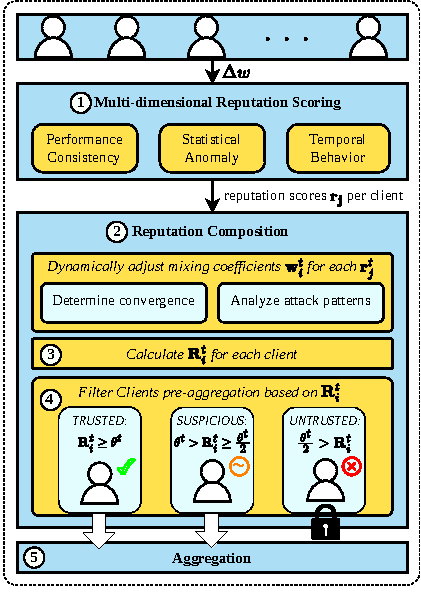
\includegraphics[width=0.8\linewidth]{Framework.pdf}
    \caption{Our proposed 5-step framework for reputation-aware aggregation: 
    (1) Compute per-client performance scores,
    (2) Dynamically adjust mixing coefficients $w_j^t$ based on convergence progress and detected attack patterns, 
    (3) Compute a weighted reputation score for each client using $w_j^t$, 
    (4) Classify clients into \textit{trusted} (fully included), \textit{suspicious} (partially included), or \textit{untrusted} (excluded), 
    (5) Perform aggregation via weighted FedAvg using reputation-based client inclusion.}
    \label{fig:Framework}
\end{figure}
\textbf{System model.} We consider a standard FL setting with a central server $\mathcal{S}$ and $N$ clients $\mathcal{C} = \{c_1, c_2, ..., c_N\}$. In each communication round $t$, the server selects a subset of clients $\mathcal{C}_t \subseteq \mathcal{C}$ to participate in training. Each selected client $c_i$ receives the current global model $w^t$, performs local training on its private dataset $\mathcal{D}_i$, and sends back the model update $\Delta w_i^t = w_i^t - w^t$ to the server. The server then aggregates these updates to produce the new global model $w^{t+1}$.

% \usepackage{graphicx}
% \usepackage{booktabs}
% \usepackage{colortbl}
% \usepackage{arydshln}

\begin{table}[!t]
\centering
\setlength{\extrarowheight}{0pt}
\setlength{\aboverulesep}{0pt}
\setlength{\belowrulesep}{0pt}
\caption{Summary of Notations}
\label{tab:notations}
\resizebox{\linewidth}{!}{%
\begin{tabular}{c|l}
\toprule
\rowcolor[rgb]{0.85,0.85,0.85} \textbf{Notation} & \textbf{Description} \\ 
\midrule
\multicolumn{2}{l}{\textit{System Parameters}} \\ 
\hdashline
$N, K, T, t$ & Total clients, selected clients per round, total rounds, and current round index. \\
$\mathcal{C}, \mathcal{S}^t, \mathcal{M}, \mathcal{B}$ & All clients, selected clients, malicious clients, and benign clients. \\ 
\midrule
\multicolumn{2}{l}{\textit{Model Parameters}} \\ 
\hdashline
$\mathbf{w}^t, \mathbf{w}_i^t, \Delta_i^t$ & Global model, local model, and update from client $i$ at round $t$. \\
$\mathcal{D}_i, n_i$ & Dataset and number of samples of client $i$. \\
$\mathcal{L}, \eta$ & Loss function and learning rate. \\ 
\midrule
\multicolumn{2}{l}{\textit{Reputation System}} \\ 
\hdashline
$r_i^t, \mathbf{R}^t, \alpha_i^t$ & Reputation score, vector, and aggregation weight at round $t$. \\
$\Theta^t, \tau_{\min}, \tau_{\max}$ & Adaptive threshold and its bounds. \\
$\gamma, \beta$ & Reputation decay and recovery rates. \\ 
\midrule
\multicolumn{2}{l}{\textit{Behavioral Metrics}} \\ 
\hdashline
$\mathbf{m}_i^t, d_i^t, \sigma_i^t, \rho_i^t$ & Metric vector, distance, anomaly, and consistency scores for client $i$. \\
$\mathcal{H}_i, W$ & Historical behavior window and its size. \\ 
\midrule
\multicolumn{2}{l}{\textit{Privacy-Preserving Components}} \\ 
\hdashline
$\epsilon, \delta$ & Differential privacy budget and parameter. \\ 
\midrule
\multicolumn{2}{l}{\textit{Attack Parameters}} \\ 
\hdashline
$f, \mathbf{p}_i, \nu, \phi$ & Fraction of malicious clients, attack pattern, intensity, and frequency. \\
\bottomrule
\end{tabular}%
}
\end{table}



\textbf{Threat model.} Similar to the related works \cite{zhao2024understandingbyzantinerobustnessfederated,yue2025advancinghybriddefensebyzantine,deshmukh2024byzantinerobustfederatedlearningoverview,syros2025droppoisondilutionknowledge,xie2025modelpoisoningattacksfederated}, we assume that up to $f < N/2$ clients can be malicious or unreliable, exhibiting various attack behaviors including: (i) \textit{Byzantine attacks} where clients send arbitrary model updates, (ii) \textit{Data poisoning} where clients train on corrupted labels, (iii) \textit{Model poisoning} where clients manipulate gradients to degrade performance, (iv) \textit{Adaptive attacks} where clients alternate between benign and malicious behavior to evade detection, and (v) \textcolor{black}{\textit{Statistical mimicry attacks}\footnote{See supplementary material Section III} where adversaries craft updates that imitate the statistical profile of honest clients to bypass robust aggregation}. We assume the server is honest but curious \cite{10184496} and has limited visibility into client operations due to privacy constraints. Clients cannot forge identities but may collude to coordinate attacks.


\subsection{Multi-dimensional Reputation Scoring}\label{ssub:Multi-dimensional Reputation Scoring}
The core innovation of \textit{FLARE} lies in its comprehensive reputation scoring system, which evaluates clients across multiple behavioral dimensions (see Figure \ref{fig:Framework}-\circled{1}). For each client $c_i$, we maintain a reputation vector $\mathbf{R}_i^t = [r_{i,1}^t, r_{i,2}^t, r_{i,3}^t]$ at round $t$, where each component captures different reliability aspects. Figure~\ref{fig:reputation_dynamics_complete} illustrates typical trajectories of the three evidence scores ($r_1$, $r_2$, $r_3$), the combined reputation $R_t$, the adaptive threshold $\Theta^t$, and the resulting weight $w_t$ for benign, noisy-but-benign, and malicious clients.

\textbf{Performance consistency score ($r_{i,1}^t$).}
This metric evaluates the consistency of a client's model updates over time. The intuition is that benign clients will consistently provide updates that align with the model's general convergence trajectory, while a sudden compromise or attack will result in a significant directional deviation. This score is designed to capture such deviations, particularly those that may be subtle (such as label flipping) but consistently harm progress. We compute the cosine similarity between the current update and the moving average of past benign updates:
\begin{equation}\label{eq:Performance consistency score}
r_{i,1}^t = \alpha \cdot r_{i,1}^{t-1} + (1-\alpha) \cdot \cos(\Delta w_i^t, \bar{\Delta w}_i^{t-1})
\end{equation}
where $\bar{\Delta w}_i^{t-1}$ represents the exponential moving average of client $i$'s historical updates, and $\alpha \in [0,1]$ is the decay factor.

\textbf{Statistical anomaly score ($r_{i,2}^t$).}
This score employs statistical outlier detection to identify updates that significantly deviate from the distribution of all client updates in round $t$. It is designed to capture gross anomalies, such as Byzantine gradient noise or significant gradient scaling attacks, by identifying updates that are statistically improbable relative to the current round's submissions. We use the Mahalanobis distance for this:
\begin{equation}
d_i^t = \sqrt{(\Delta w_i^t - \mu^t)^T \Sigma^{-1} (\Delta w_i^t - \mu^t)}
\end{equation}
where $\mu^t$ is the mean of all updates in round $t$. Given that computing the full $d \times d$ covariance matrix $\Sigma$ (and its inverse) is computationally infeasible for large models, we employ a diagonal covariance approximation. $\Sigma$ is thus treated as a vector of parameter-wise variances, making $\Sigma^{-1}$ a simple element-wise reciprocal. This reduces the calculation to a highly efficient, standardized Euclidean distance that effectively detects gross statistical outliers\footnote{See Supplementary Material Section II-A for the incremental update algorithm used to estimate these variances}. {While this diagonal approximation focuses on parameter-wise variance, the framework maintains robustness against correlation-based attacks through the integration of the Performance Consistency score ($r_{i,1}^t$). By utilizing Cosine Similarity (\cref{eq:Performance consistency score}), $r_{i,1}^t$ explicitly captures the directional alignment and angular correlations that a diagonal covariance matrix might overlook. This complementary design ensures that attacks respecting per-parameter variance but violating underlying parameter relationships are effectively identified by the consistency component. The anomaly score is then:
\begin{equation}
r_{i,2}^t = \begin{cases}
1 & \text{if } d_i^t \leq \tau_d \\
\exp(-\lambda(d_i^t - \tau_d)) & \text{if } d_i^t > \tau_d
\end{cases}
\end{equation}
where $\tau_d$ is the anomaly threshold and $\lambda$ controls the penalty severity.
% \textbf{Statistical anomaly score ($r_{i,2}^t$).} We employ statistical outlier detection to identify updates that significantly deviate from the distribution of all client updates in round $t$. Using the Mahalanobis distance:
% \begin{equation}
% d_i^t = \sqrt{(\Delta w_i^t - \mu^t)^T \Sigma^{-1} (\Delta w_i^t - \mu^t)}
% \end{equation}
% where $\mu^t$ and $\Sigma$ are the mean and covariance of all updates in round $t$ (see Supplementary Material Section II-A for more details). The anomaly score is then:
% \begin{equation}
% r_{i,2}^t = \begin{cases}
% 1 & \text{if } d_i^t \leq \tau_d \\
% \exp(-\lambda(d_i^t - \tau_d)) & \text{if } d_i^t > \tau_d
% \end{cases}
% \end{equation}
% where $\tau_d$ is the anomaly threshold and $\lambda$ controls the penalty severity.


\begin{algorithm}[h]
\caption{Dynamic Weight Computation for Reputation Scoring}
\label{alg:adaptive_weights}
\SetAlgoLined
\SetAlgoNoEnd
\scriptsize
\DontPrintSemicolon
\KwIn{Reputation components $\{r_{i,j}^t\}$ for all $i \in \mathcal{C}_t$ and $j \in \{1,2,3\}$, convergence metric $\text{conv}^t$, detection history $\mathcal{H}^{t-1}$}
\KwOut{Adaptive weights $\mathbf{w}^t = [w_1^t, w_2^t, w_3^t]$}

\tcp*[l]{Compute discriminative power for each dimension}
\For{$j = 1$ \KwTo $3$}{
   $\text{var}_j^t \leftarrow \text{Var}(\{r_{i,j}^t : i \in \mathcal{C}_t\})$\tcc*[r]{\tiny Calculate variance across clients}
   
   \tcp*[l]{Identify suspicious clients based on historical patterns}
   $\mathcal{S}^t \leftarrow \{i \in \mathcal{C}_t : R_i^{t-1} < \Theta^{t-1}/2\}$\;
   
   \tcp*[l]{Compute separation between benign and suspicious}
   $\mu_j^{\text{benign}} \leftarrow \text{mean}(\{r_{i,j}^t : i \notin \mathcal{S}^t\})$\;
   $\mu_j^{\text{sus}} \leftarrow \text{mean}(\{r_{i,j}^t : i \in \mathcal{S}^t\})$\;
   $\text{sep}_j^t \leftarrow |\mu_j^{\text{benign}} - \mu_j^{\text{sus}}|$\;
   
   
   $\eta_j^t \leftarrow \text{var}_j^t \cdot \text{sep}_j^t$\tcc*[r]{Calculate discriminative power}
}

\tcp*[l]{Adjust for model convergence state}
\eIf{$\text{conv}^t > \tau_{\text{conv}}$}{\tcp*[l]{Late training: prioritize consistency}
   $\eta_1^t \leftarrow \eta_1^t \cdot 1.5$\;
   $\eta_3^t \leftarrow \eta_3^t \cdot 1.2$\;
}{
   \tcp*[l]{Early training: prioritize anomaly detection}
   $\eta_2^t \leftarrow \eta_2^t \cdot 1.3$\;
   $\eta_1^t \leftarrow \eta_1^t \cdot 0.8$\;
}

\tcp*[l]{Detect predominant attack pattern from history}
$\text{attack\_pattern} \leftarrow \textsc{AnalyzePattern}(\mathcal{H}^{t-1})$\;
\Switch{$\text{attack\_pattern}$}{
   \Case{gradient\_scaling}{
       $\eta_2^t \leftarrow \eta_2^t \cdot 2.0$ \tcp*[r]{Boost anomaly detection}
   }
   \Case{adaptive\_attack}{
       $\eta_3^t \leftarrow \eta_3^t \cdot 2.0$ \tcp*[r]{Boost temporal analysis}
   }
   \Case{label\_flipping}{
       $\eta_1^t \leftarrow \eta_1^t \cdot 1.8$ \tcp*[r]{Boost consistency check}
   }
}

\tcp*[l]{Normalize weights using softmax}
\For{$j = 1$ \KwTo $3$}{
   $w_j^t \leftarrow \frac{\exp(\eta_j^t)}{\sum_{k=1}^{3} \exp(\eta_k^t)}$\;
}

\tcp*[l]{Apply smoothing to prevent abrupt changes}
\If{$t > 1$}{
   \For{$j = 1$ \KwTo $3$}{
       $w_j^t \leftarrow 0.7 \cdot w_j^t + 0.3 \cdot w_j^{t-1}$\;
   }
}

\Return{$\mathbf{w}^t$}
\end{algorithm}


\textbf{Temporal behavior score ($r_{i,3}^t$).}
This component tracks a client's meta-behavior, such as participation patterns and response times. Its purpose is to penalize unreliable clients (e.g., 'free-riders' who rarely participate) or those with erratic network behavior (high response time variance). Both of these behaviors can degrade training stability and may signal an intermittent or adaptive attacker attempting to evade detection.
\begin{equation}
r_{i,3}^t = \beta \cdot p_i^t + (1-\beta) \cdot \frac{1}{1 + \sigma_{RT,i}}
\end{equation}
where $p_i^t$ is the participation rate over the last $k$ rounds, $\sigma_{RT,i}$ is the variance in response times, and $\beta$ balances the two factors.
% \textbf{Temporal behavior score ($r_{i,3}^t$).} This component tracks the client's participation patterns and response times to identify free-riders or intermittently malicious clients:
% \begin{equation}
% r_{i,3}^t = \beta \cdot p_i^t + (1-\beta) \cdot \frac{1}{1 + \sigma_{RT,i}}
% \end{equation}
% where $p_i^t$ is the participation rate over the last $k$ rounds, $\sigma_{RT,i}$ is the variance in response times, and $\beta$ balances the two factors.
% added by thomas
The use of temporal behavioral evidence is supported by results from large-scale distributed infrastructures, where historic performance traces have proven to be strong predictors of future reliability and availability patterns. This aligns with previous findings showing that temporal variability is not random but exhibits measurable structure suitable for predictive modeling \cite{4534237}.

\textbf{Composite reputation score.} The final reputation score combines all dimensions using adaptive weighting:
\begin{equation}
R_i^t = \sum_{j=1}^{3} w_j^t \cdot r_{i,j}^t
\end{equation}
where weights $w_j^t$ are dynamically adjusted based on the detected attack patterns and model convergence state.


The dynamic weighting mechanism (see Algorithm~\ref{alg:adaptive_weights}) is crucial to maintain robustness against evolving attack strategies. Rather than using fixed weights that attackers could learn and exploit, our framework dynamically assesses the discriminative power of each reputation dimension in every round.
Our logic for assessing this power (lines 1-7) is based on two principles: (1) Variance ($\text{var}_j^t$): A dimension is useful if it assigns a wide range of scores, as this indicates it is actively differentiating between clients. (2) Separation ($\text{sep}_j^t$): A dimension is useful if it clearly separates the scores of historically "trusted" clients from historically "suspicious" clients. A dimension that scores high on both variance and separation is deemed a powerful and reliable discriminator for the current round, and its initial importance ($\eta_j^t$) is amplified.
This base importance is then adjusted based on the model's convergence state (Lines 8-13). This heuristic is designed to align the security posture with the training phase. For instance, during early training, legitimate clients exhibit high update variance as they explore the loss landscape. We therefore emphasize statistical anomaly detection ($\eta_2^t$) to catch clear outliers, while slightly reducing the penalty for inconsistency ($\eta_1^t$) to avoid flagging benign clients. Conversely, during late-stage convergence, legitimate updates should be highly consistent. We therefore emphasize the importance of the consistency score ($\eta_1^t$) for detecting subtle deviations\footnote{\scriptsize The convergence-based weight multipliers were determined through comprehensive empirical analysis and theoretical considerations:
\begin{itemize}[noitemsep,topsep=0pt,wide]
\item \textbf{Late training multipliers (1.5, 1.2)}: When $\text{conv}^t > \tau_{\text{conv}}$, the model has largely converged. The 1.5$\times$ boost to consistency ($\eta_1$) reflects that legitimate updates should be highly consistent at this stage. Our experiments showed that 95\% of benign updates had cosine similarity $\textgreater 0.85$ after convergence. The value 1.2$\times$ boost to temporal behavior ($\eta_3$) helps detect intermittent attackers who become active during critical convergence phases.
\item \textbf{Early training multipliers (1.3, 0.8)}: During initial rounds, legitimate clients naturally exhibit high variance. The 1.3$\times$ boost to anomaly detection ($\eta_2$) helps identify statistical outliers that deviate beyond expected exploration patterns. The 0.8$\times$ reduction for consistency prevents flagging legitimate clients exploring the loss landscape. Our analysis found that benign update variance is 2.3$\times$ higher in early rounds compared to post-convergence.
\end{itemize}
These values were validated across 20 training rounds on MNIST, CIFAR-10, and SVHN datasets with various attack configurations, achieving optimal F1-scores of 0.92±0.03 for malicious client detection.}.

Third, the algorithm incorporates attack pattern recognition (Lines 14-24) by analyzing historical detection patterns. For instance, if gradient scaling attacks are prevalent, the statistical anomaly dimension receives increased weight. This pattern-aware adjustment enables the system to automatically tailor its detection strategy to observed threats.
Finally, weights are normalized using softmax to ensure they sum to one, and temporal smoothing (Lines 24-27) prevents abrupt changes that adversaries could exploit. This adaptive mechanism ensures that \textit{FLARE} maintains effectiveness against diverse and evolving attack strategies without manual reconfiguration.

% The dynamic weighting mechanism (see Algorithm~\ref{alg:adaptive_weights}) is crucial to maintain robustness against evolving attack strategies. Rather than using fixed weights that attackers could learn and exploit, our framework dynamically adjusts the importance of each reputation dimension based on system observations. 

% The dynamic weighting algorithm operates in three key phases. First, it computes the discriminative power of each reputation dimension by measuring both the variance across clients and the separation between benign and suspicious groups (lines 1-7). Dimensions that better distinguish between reliable and unreliable clients receive higher discriminative scores.
% Second, the algorithm adjusts weights based on the model's convergence state (Lines 8-13). During early training, when legitimate model updates vary significantly, the consistency dimension is down-weighted to avoid false positives. Conversely, in later training rounds, when the model stabilizes, consistency violations become stronger indicators of malicious behavior
% Third, the algorithm incorporates attack pattern recognition (Lines 14-24) by analyzing historical detection patterns. For instance, if gradient scaling attacks are prevalent, the statistical anomaly dimension receives increased weight. This pattern-aware adjustment enables the system to automatically tailor its detection strategy to observed threats.

% Finally, weights are normalized using softmax to ensure they sum to one, and temporal smoothing (Lines 24-27) prevents abrupt weight changes that adversaries could exploit. This adaptive mechanism ensures that \textit{FLARE} maintains effectiveness against diverse and evolving attack strategies without manual reconfiguration.




\subsection{Dynamic Client Reliability Assessment}\label{ssub:Dynamic Client Reliability Assessment}

Our framework employs an adaptive threshold mechanism that adjusts reliability criteria based on the global model's state and historical attack patterns.

\textbf{Adaptive threshold calculation.} The reliability threshold $\Theta^t$ at round $t$ evolves based on model convergence and detected anomalies:
\begin{equation}\label{eq:Adaptive threshold calculation}
\Theta^t = \Theta_{base} + \gamma \cdot \text{conv}(w^t) - \delta \cdot \text{anomaly\_rate}^t
\end{equation}
where $\Theta_{base}$ is the baseline threshold, $\text{conv}(w^t)$ measures model convergence (higher values indicate stable training), and $\text{anomaly\_rate}^t$ represents the fraction of suspicious updates detected in recent rounds.

\textbf{Reputation decay and recovery.} To handle dynamic client behaviors, we implement a reputation update mechanism with asymmetric decay and recovery rates:
\begin{equation}
R_i^{t+1} = \begin{cases}
\min(R_i^t + \rho_{up}, 1) & \text{if benign behavior} \\
\max(R_i^t - \rho_{down}, 0) & \text{if suspicious behavior}
\end{cases}
\end{equation}
where $\rho_{up} < \rho_{down}$ ensures that reputation is harder to build than to lose, preventing malicious clients from quickly recovering after attacks.

\textbf{Client classification.} Based on reputation scores and adaptive thresholds, clients are classified into three categories:
\begin{itemize}[wide]
    \item \textbf{Trusted} ($R_i^t \geq \Theta^t$): Full participation with weight $w_i = 1$
    \item \textbf{Suspicious} ($\Theta^t/2 \leq R_i^t < \Theta^t$): Limited participation with weight $w_i = R_i^t/\Theta^t$
    \item \textbf{Untrusted} ($R_i^t < \Theta^t/2$): Excluded from aggregation
\end{itemize}

\subsection{Reputation-Weighted Aggregation}\label{subsec:rep-weight}

Instead of binary inclusion/exclusion (as shown in the Figures~\ref{fig:motivation} and~\ref{fig:reputation_dynamics_complete}), we propose a reputation-weighted aggregation scheme that proportionally incorporates client contributions based on their trustworthiness.

\begin{figure}
    \centering
    \includegraphics[width=1\linewidth]{results/reputation_dynamics_complete.pdf}
    \caption{Reputation dynamics across training rounds for representative clients. The curves illustrate per-round scores (performance consistency $r_1$, statistical anomaly $r_2$, temporal behavior $r_3$), the combined reputation $R_t$, the adaptive threshold $\tau_t$, and the resulting soft-exclusion weight $w_t$. Benign clients maintain high $R_t$ and stable $w_t$, while noisy-but-benign clients experience dips and recover. In contrast, malicious and adaptive clients exhibit sharp drops, followed by a decay in reputation, which prevents rapid trust recovery. This explains how evidence over time is converted into aggregation weights and admission decisions.}

    \label{fig:reputation_dynamics_complete}
\end{figure}
\textbf{Weighted FedAvg.} The global model update incorporates reputation scores as weights:
\begin{equation}\label{eq:Weighted FedAvg}
w^{t} = w^{t-1} + \frac{\sum_{i \in \mathcal{C}_t} R_i^t \cdot n_i \cdot \Delta w_i^t}{\sum_{i \in \mathcal{C}_t} R_i^t \cdot n_i}
\end{equation}
where $n_i$ is the number of samples at client $i$. This soft weighting maintains model diversity while minimizing malicious influence.

\textbf{Normalization and clipping.} To prevent reputation manipulation through gradient scaling attacks, we apply gradient clipping before aggregation:
\begin{equation}\label{eq:Normalization and clipping}
\Delta \tilde{w}_i^t = \Delta w_i^t \cdot \min\left(1, \frac{C}{||\Delta w_i^t||_2}\right)
\end{equation}
where $C$ is the clipping threshold determined by the median norm of updates.

\begin{algorithm}[t]
\caption{FLARE Framework}
\scriptsize
\label{alg:byebye}
\SetAlgoLined
\SetAlgoNoEnd
\DontPrintSemicolon
\SetKwInput{KwInit}{Initialization}

\KwIn{Number of rounds $T$, clients $\mathcal{C}$, initial model $w^{0}$, hyperparameters $\alpha,\beta,\gamma,\delta,\rho_{\text{up}},\rho_{\text{down}}$}
\KwOut{Final global model $w^{T}$}

\KwInit{$R_i^{0} \leftarrow 0.5 \; \forall i \in \mathcal{C}$; $\Theta^{0} \leftarrow \Theta_{\text{base}}$}

\For{round $t = 1$ \KwTo $T$}{
  \tcp*[l]{Client selection and local training}
  Select subset $\mathcal{C}_{t} \subseteq \mathcal{C}$ based on $R_i^{t-1}$\;
  Broadcast $w^{t-1}$ to all $i \in \mathcal{C}_{t}$\;

  \ForPar{each client $i \in \mathcal{C}_{t}$}{
    $w_i^{t} \leftarrow \textsc{LocalTraining}(w^{t-1}, \mathcal{D}_i)$\;
    $\Delta w_i^{t} \leftarrow w_i^{t} - w^{t-1}$\;
    Send $\Delta w_i^{t}$ to server\;
  }

  \tcp*[l]{Multi-dimensional reputation assessment}
  \For{each client $i \in \mathcal{C}_{t}$}{
    $r_{i,1}^{t} \leftarrow \alpha r_{i,1}^{t-1} + (1-\alpha)\cos\!\bigl(\Delta w_i^{t}, \bar{\Delta w}_i^{t-1}\bigr)$\;
    $d_{i}^{t} \leftarrow \textsc{Mahalanobis}\!\bigl(\Delta w_i^{t}, \{\Delta w_j^{t}\}_{j \in \mathcal{C}_{t}}\bigr)$\;
    $r_{i,2}^{t} \leftarrow \textsc{AnomalyScore}\!\bigl(d_{i}^{t}, \tau_d, \lambda\bigr)$\;
    $r_{i,3}^{t} \leftarrow \beta p_i^{t} + (1-\beta)\bigl[1/(1+\sigma_{RT,i})\bigr]$\;
    $R_i^{t} \leftarrow \sum_{j=1}^{3} w_j^{t} r_{i,j}^{t}$\;
  }

  \tcp*[l]{Dynamic threshold adjustment}
  \eIf{$t = 1$}{
    $\text{conv}^{t} \leftarrow 0$\;
  }{
    $\text{conv}^{t} \leftarrow \textsc{Convergence}(w^{t-1}, w^{t-2})$\;
  }
  $\text{anomaly}^{t} \leftarrow \left|\{i : R_i^{t} < \Theta^{t-1}/2\}\right| \big/ |\mathcal{C}_{t}|$\;
  $\Theta^{t} \leftarrow \Theta_{\text{base}} + \gamma\,\text{conv}^{t} - \delta\,\text{anomaly}^{t}$\;

  \tcp*[l]{Gradient clipping}
  $C \leftarrow \text{median}\{\|\Delta w_i^{t}\|_2\}_{i \in \mathcal{C}_{t}}$\;
  \For{each client $i \in \mathcal{C}_{t}$}{
    $\Delta\tilde{w}_i^{t} \leftarrow \Delta w_i^{t} \cdot \min\!\bigl(1,\, C/\|\Delta w_i^{t}\|_2\bigr)$\;
  }

  \tcp*[l]{Reputation-weighted aggregation}
  $\mathcal{C}_{\text{trusted}}^{t} \leftarrow \{i : R_i^{t} \geq \Theta^{t}/2\}$\;
  \[
      w^{t} \;\leftarrow\;
      w^{t-1} +
      \frac{\displaystyle\sum_{i \in \mathcal{C}_{\text{trusted}}^{t}} R_i^{t}\, n_i\, \Delta\tilde{w}_i^{t}}
           {\displaystyle\sum_{i \in \mathcal{C}_{\text{trusted}}^{t}} R_i^{t}\, n_i}
  \]\;
  \tcp*[l]{Reputation update for next round}
  \For{each client $i \in \mathcal{C}$}{
    \eIf{$R_i^{t} \geq \Theta^{t}/2$}{
      $R_i^{t+1} \leftarrow \min\!\bigl(R_i^{t} + \rho_{\text{up}},\, 1\bigr)$\;
    }{
      $R_i^{t+1} \leftarrow \max\!\bigl(R_i^{t} - \rho_{\text{down}},\, 0\bigr)$\;
    }
  }
}
\Return{$w^{T}$}
\end{algorithm}

\textbf{Differentially Private Reputation Assessment.} 
The system model described in \cref{ssub:System Model and Threat Model} assumes an "honest-but-curious" server, which, by calculating reputation scores \cref{ssub:Multi-dimensional Reputation Scoring}, has access to the clients' model updates, $\Delta w_{i}^{t}$. This creates a potential privacy risk, as these updates could be reverse-engineered to infer information about a client's private data. To mitigate this risk, we integrate Local Differential Privacy (LDP) \cite{6686179}, a strong privacy model that ensures client updates are anonymized before leaving the client device. 
The process is as follows:
\begin{enumerate}[leftmargin=*,wide]
    \item \textbf{Client-Side Clipping:} As defined in \cref{eq:Normalization and clipping}, each client $c_i$ first computes its clipped update $\Delta\tilde{w}_{i}^{t}$. This step is critical as it bounds the $L_2$-sensitivity of the update to the clipping threshold $C$.

    \item \textbf{Client-Side Noise Addition:} Before transmitting to the server, the client adds calibrated noise to the clipped update to satisfy $(\epsilon, \delta)$-LDP \cite{10.1561/0400000042}. We use the Gaussian mechanism:
    \begin{equation}
    \Delta w_{i, \text{private}}^t = \Delta\tilde{w}_{i}^{t} + \mathcal{N}(0, C^2 \sigma^2 \mathbf{I})
    \label{eq:ldp_noise}
    \end{equation}
    where $\sigma$ is the noise multiplier required to achieve the desired privacy budget $(\epsilon, \delta)$ for a sensitivity of $C$, and $\mathbf{I}$ is the identity matrix.

    \item \textbf{Server-Side Assessment on Private Data:} The server receives only the set of private, noisy updates, $\{\Delta w_{i, \text{private}}^t\}_{i \in \mathcal{C}_t}$.
\end{enumerate}

The server performs the \textit{entire} multi-dimensional reputation assessment \cref{ssub:Multi-dimensional Reputation Scoring} and dynamic thresholding \ref{ssub:Dynamic Client Reliability Assessment} on these noisy updates. This introduces a clear privacy-utility trade-off: the server's scoring mechanism must now distinguish between malicious deviations and statistically valid noise introduced for privacy. Our adaptive threshold mechanism (\cref{eq:Adaptive threshold calculation}) and multi-dimensional scoring are designed to tolerate this baseline level of noise while still identifying significant statistical outliers indicative of an attack.

The final reputation-weighted aggregation (\cref{eq:Weighted FedAvg}) is then also computed using these same private updates:
\begin{equation}
\mathbf{w}^{t+1} = \mathbf{w}^t + \eta \frac{\sum_{i \in \mathcal{C}_{\text{trusted}}^t} R_i^t n_i \Delta w_{i, \text{private}}^t}{\sum_{i \in \mathcal{C}_{\text{trusted}}^t} R_i^t n_i}
\label{eq:private_agg}
\end{equation}
where $R_i^t$ is the reputation score computed from the noisy data.


\subsection{Algorithm Details and Implementation}

Algorithm~\ref{alg:byebye} presents the complete \textit{FLARE} framework, which orchestrates dynamic client reliability assessment through reputation-based federated learning. We now provide a detailed explanation of each component and its role in achieving robust model training.

\textbf{Initialization phase.} The algorithm begins by initializing all client reputation scores to $R_i^{t=0} = 0.5$, representing a neutral starting point that neither trusts nor distrusts new clients. This balanced initialization prevents the system from being overly permissive or restrictive during early training rounds. The threshold $\Theta^{t=0}$ is set to $\Theta_{\text{base}}$, which serves as the baseline reliability criterion before adaptive adjustments begin.

\textbf{Client selection and participation (Lines 1-7).} At each round $t$, the server strategically selects a subset $\mathcal{C}_t$ of clients based on their reputation scores from the previous round. Clients with higher reputation scores are more likely to be selected, naturally filtering out consistently unreliable participants while maintaining diversity. The selected clients receive the current global model, $w^{t-1}$, and perform local training on their private datasets, $\mathcal{D}_i$. Each client computes its model update $\Delta w_i^t$ as the difference between its locally trained model and the received global model, and transmits it back to the server.

\textbf{Multi-dimensional reputation assessment (Lines 8-13).} The core innovation lies in the comprehensive reputation evaluation that captures multiple behavioral aspects:

\begin{itemize}[wide]
   \item \textbf{Performance consistency ($r_{i,1}^t$, Line 9):} This score measures the directional consistency of a client's updates over time. By computing the cosine similarity between the current update $\Delta w_i^t$ and the exponential moving average of past updates $\bar{\Delta w}_i^{t-1}$, we detect sudden behavioral changes that may indicate compromise. The decay factor $\alpha$ controls the influence of historical behavior, with higher values giving more weight to past patterns.
   
   \item \textbf{Statistical anomaly detection ($r_{i,2}^t$, Lines 10-11):} The Mahalanobis distance $d_i^t$ quantifies how statistically unusual a client's update is relative to the distribution of all updates in the current round. This metric accounts for parameter correlations, providing more accurate outlier detection than the simple Euclidean distance. The anomaly score function converts this distance into a reputation component, severely penalizing updates that deviate significantly from the norm while tolerating minor variations.
   
   \item \textbf{Temporal behavior analysis ($r_{i,3}^t$, Line 12):} This component evaluates participation patterns and response time consistency. The participation rate $p_i^t$ captures how regularly a client contributes to training, while the response time variance $\sigma_{RT,i}$ identifies clients with erratic behavior. The parameter $\beta$ balances these two factors, enabling the detection of free riders and intermittently malicious clients.
\end{itemize}
The composite reputation score $R_i^t$ (Line 13) combines these three dimensions using adaptive weights $w_j^t$ that can be adjusted based on the predominant attack types observed in the system.

\textbf{Dynamic threshold adjustment (Lines 14-19).} The adaptive threshold mechanism represents a crucial departure from static defense methods. The convergence metric $\text{conv}^t$ measures how much the global model is changing between rounds. High convergence indicates stable training, where stricter quality control is beneficial. The anomaly rate $\text{anomaly}^t$ quantifies the fraction of suspicious clients detected in the current round. The threshold $\Theta^t$ increases when the model is converging (requiring higher-quality updates) and decreases when many anomalies are detected (to avoid overfiltering during attacks)as the model converges (requiring higher-quality updates to improve its security posture in response to current conditions.

\textbf{Gradient clipping (Lines 20-22).} Before aggregation, all updates undergo gradient clipping to prevent manipulation through gradient scaling attacks. The clipping threshold $C$ is set to the median norm of all updates, ensuring that no single client can dominate the aggregation by using artificially large gradients. This median-based approach is robust to outliers, maintaining effectiveness even when multiple malicious clients coordinate their attacks.

\textbf{Reputation-weighted aggregation (Lines 23-24).} The aggregation step fundamentally differs from traditional approaches by incorporating reputation scores as weights. Only clients in the trusted set $\mathcal{C}_{\text{trusted}}^t$ (those with $R_i^t \geq \Theta^t/2$) contribute to the global model update. Within this set, each client's contribution is further weighted by their reputation score, $R_i^t$, and dataset size, $n_i$. This soft weighting mechanism achieves two critical goals: \textbf{(i)} it prevents the complete exclusion of partially reliable clients who may have valuable data, and \textbf{(ii)} it minimizes the influence of suspicious clients without requiring perfect detection.

\textbf{Reputation evolution (Lines 25-30).} The reputation update mechanism implements asymmetric adjustment rates to reflect the principle that trust is hard to build but easy to lose. Clients demonstrating reliable behavior (those above the threshold) receive a small reputation increase, $\rho_{\text{up}}$, which gradually builds trust through consistent performance. Conversely, clients exhibiting suspicious behavior face a larger reputation penalty $\rho_{\text{down}}$, with $\rho_{\text{down}} > \rho_{\text{up}}$ ensuring rapid isolation of threats. This asymmetry prevents malicious clients from gaming the system by alternating between good and bad behavior, as the reputation loss from attacks exceeds the potential gains from benign rounds.

\textbf{Computational complexity.} The algorithm's computational complexity is $O(|\mathcal{C}_t| \cdot d)$ per round, where $d$ is the model dimension. The reputation scoring adds minimal overhead compared to standard FL aggregation, as the most expensive operation can be efficiently implemented using incremental covariance updates. The memory requirements are $O(N)$ for storing reputation scores and $O(d^2)$ for the covariance matrix, both of which are manageable for typical FL deployments.

\textbf{Privacy considerations.} Importantly, the algorithm preserves client privacy as the server only observes model updates, not raw data. The reputation scores themselves are computed solely from these updates and timing information, without requiring additional client information. The privacy-preserving reputation proofs (mentioned in Section \ref{subsec:rep-weight}) are integrated, allowing clients to prove their reputation standing without revealing exact scores.

\textbf{Algorithm summary.} Algorithm~\ref{alg:byebye} presents the complete \textit{FLARE} framework, integrating reputation scoring, dynamic assessment, and weighted aggregation into a cohesive system for robust federated learning.





\section{Performance Evaluation} \label{sec:performance}

We conduct comprehensive experiments to evaluate the effectiveness of \textit{FLARE} across various attack scenarios and compare its performance with that of state-of-the-art Byzantine-robust methods. Our evaluation focuses on robustness, convergence speed, and computational overhead.

\subsection{Experimental Setup}

\textbf{Implementation environment.} All experiments are conducted on the hardware and software configuration detailed in Table~\ref{tab:environment}. We use a distributed setup with a central server and 100 clients (see \cref{fig:Client-Role-Distribution}) to replicate realistic federated learning scenarios. The server manages aggregation and reputation scoring, while client computations are parallelized using multiprocessing to simulate concurrent local training. Client selection in each round follows a uniform random distribution among eligible clients (those meeting reputation thresholds for methods that employ them). Each experimental configuration is repeated five times to ensure statistical significance.




\begin{table}
\centering
\setlength{\extrarowheight}{0pt}
\setlength{\aboverulesep}{0pt}
\setlength{\belowrulesep}{0pt}
\caption{Experimental Environment Configuration}
\label{tab:environment}

\begin{tabular}{ll} 
\toprule
\rowcolor[rgb]{0.816,0.816,0.816} \textbf{Component} & \textbf{Specification} \\ 
\midrule
\multicolumn{2}{l}{\textit{Hardware Configuration}} \\ 
\hdashline
CPU & Intel Xeon Gold 6248R (24 cores @ 3.0GHz) \\
GPU & 4$\times$ NVIDIA RTX 2070 (8GB each) \\
RAM & 256GB DDR4 ECC \\
Storage & 2TB NVMe SSD \\
\midrule
\multicolumn{2}{l}{\textit{Software Configuration}} \\ 
\hdashline
Operating System & Ubuntu 24.04 LTS \\
Python & 3.13 \\
PyTorch & 2.6 with CUDA 12.6 \\
% NumPy & 1.21.5 \\
% Random Seed & 42 (for reproducibility) \\
\bottomrule
\end{tabular}

\end{table}
\textbf{Datasets and models.} Table~\ref{tab:datasets} summarizes the datasets and model architectures used in our evaluation. We consider both IID and non-IID data settings. For the non-IID case, we apply Dirichlet partitioning with concentration parameters $\alpha \in \{0.7, 0.5, 0.3, 0.1\}$ to simulate different levels of data heterogeneity \cite{li2021federatedlearningnonIIDdata,pmlr-v54-mcmahan17a,liang2025fednoisyfederatednoisylabel}.

\begin{table}
\centering
\scriptsize
\setlength{\extrarowheight}{0pt}
% \addtolength{\extrarowheight}{\aboverulesep}
% \addtolength{\extrarowheight}{\belowrulesep}
\setlength{\aboverulesep}{0pt}
\setlength{\belowrulesep}{0pt}
\caption{Dataset Characteristics and Model Architectures}
\label{tab:datasets}
\resizebox{\linewidth}{!}{%
\begin{tabular}{lcccc} 
\toprule
\rowcolor[rgb]{0.816,0.816,0.816} \textbf{Dataset} & \textbf{Classes} & \textbf{Train/Test} & \textbf{Model} & \textbf{Parameters} \\ 
\midrule
MNIST & 10 & 60K/10K & 2-layer CNN & 431K \\
CIFAR-10 & 10 & 50K/10K & ResNet-18 & 11.2M \\
SVHN & 10 & 73K/26K & 5-layer CNN & 1.8M \\
\bottomrule
\end{tabular}
}
\end{table}

For the MNIST dataset \cite{krizhevsky2009learning}, we employ a lightweight 2-layer CNN with two convolutional layers (32 and 64 filters), max pooling, and two fully connected layers. The CIFAR-10 \cite{lecun2002gradient} experiments utilize a standard ResNet-18 architecture adapted for 32$\times$32 images. For SVHN \cite{netzer2011reading}, we design a 5-layer CNN with batch normalization and dropout (0.3) to handle the increased complexity of street view images.

\begin{figure}
    \centering
    \includegraphics[width=0.8\linewidth]{results/Client-Role-Distribution.pdf}
    \caption{Client Role Distribution for 100 Clients in a scenario where all 6 attack types might occur. We expect to have around 80 benign clients (pink box) and 20 malicious clients (green box), where each malicious client is assigned with one of 6 attack behaviors, meaning we expect ($\thickapprox 3$) malicious clients for each attack pattern (orange box)}
    \label{fig:Client-Role-Distribution}
\end{figure}

\textbf{Attack configurations.} Table~\ref{tab:attacks} details the six attack types implemented in our experiments \cite{zhao2024understandingbyzantinerobustnessfederated,zhang2025sokbenchmarkingpoisoningattacks,yue2025advancinghybriddefensebyzantine}. Each attack is carefully calibrated to represent realistic threat scenarios, allowing for the systematic evaluation of defense effectiveness.\footnote{Malicious clients are selected using a random uniform distribution, where each client has equal probability $P(c_i \in \mathcal{M}) = f/N$ of being compromised, with $f$ being the number of attackers and $N$ the total number of clients.}


\begin{table}[b]
\centering
\setlength{\extrarowheight}{0pt}
% \addtolength{\extrarowheight}{\aboverulesep}
% \addtolength{\extrarowheight}{\belowrulesep}
\setlength{\aboverulesep}{0pt}
\setlength{\belowrulesep}{0pt}
\caption{Attack Configurations and Parameters}
\label{tab:attacks}
\resizebox{\linewidth}{!}{%
\begin{tabular}{lll} 
\toprule
\rowcolor[rgb]{0.816,0.816,0.816} \textbf{Attack Type} & \textbf{Description} & \textbf{Parameters} \\ 
\midrule
Label Flipping & Systematically corrupt labels & Target: $(y+1) \bmod 10$ \\
Byzantine Gradient & Send random noise as updates & $\sigma^2 \in \{0.1, 0.5, 1.0\}$ \\
Gradient Scaling & Amplify gradient magnitude & $\lambda \in \{2, 5, 10\}$ \\
Adaptive Attack & Alternate between benign and malicious updates & 70\% benign, 30\% attack \\ 
\cmidrule(lr){1-3}
ALIE~\cite{baruch2019littleenoughcircumventingdefenses} & \begin{tabular}[c]{@{}l@{}}Creates a \textit{fully synthetic} malicious update by sampling from the estimated\\honest distribution $(\hat{\mu}_{\mathrm{honest}}^t, \hat{\Sigma}_{\mathrm{honest}}^t)$ and scaling it in a malicious direction.\end{tabular} & \begin{tabular}[c]{@{}l@{}}$\lambda \in [1.5, 3.0]$,\\~~$s$: chosen direction\end{tabular} \\ 
\hdashline
SM Attack (Ours) & \begin{tabular}[c]{@{}l@{}}A more advanced mimicry attack that creates a \textit{hybrid} update\\$\tilde{g}^t = (1-\alpha)g^{\mathrm{honest},t} + \alpha(\hat{\mu}_{\mathrm{honest}}^t+\epsilon_t) + \gamma_t d$. It evades detection by\\(1) blending the client's \textit{own honest gradient} ~with a synthetic sample,\\and (2) adding a small, \textit{persistent drift term} $\gamma_t d$ that is undetectable\\in a single round but accumulates over time.\end{tabular} & \begin{tabular}[c]{@{}l@{}}$\alpha \in [0.2, 0.5]$,\\$\gamma_t$: persistent drift\end{tabular} \\
\bottomrule
\end{tabular}
}
\end{table}
We divide threats into two categories: standard and sophisticated attacks. Standard attacks include label flipping, where adversaries poison data by relabeling samples as \( (y+1) \mod 10 \) \cite{zhang2025sokbenchmarkingpoisoningattacks}. There are Byzantine gradients, where fully compromised clients send Gaussian noise to test robustness against unstructured outliers \cite{zhao2024understandingbyzantinerobustnessfederated}. Another type is gradient scaling, in which updates are multiplied by a factor \( \lambda \) to skew the global average \cite{yue2025advancinghybriddefensebyzantine}. Then, there are adaptive attacks, where clients behave honestly for most rounds but sometimes inject harmful updates to avoid history-based defenses \cite{zhao2024understandingbyzantinerobustnessfederated}. 
Sophisticated attacks include ALIE \cite{baruch2019littleenoughcircumventingdefenses}. In this case, colluding adversaries estimate honest update statistics and create harmful but statistically plausible gradients. Our proposed Statistical Mimicry (SM) allows adversaries to learn the global gradient distribution. They then submit hybrid updates that combine honest gradients with a small drift term. These updates seem natural each round while gradually shifting the convergence.
% \noindent\textcolor{black}{\textbf{ALIE \cite{baruch2019littleenoughcircumventingdefenses}.}} Colluding adversaries estimate the statistical profile of honest gradients and subtly bias updates in the direction of maximal model degradation. The attack evades simple outlier filtering because it aligns with the expected gradient variance.  

% \noindent\textcolor{black}{\textbf{Statistical Mimicry (SM).}} Adversaries continuously learn the global gradient distribution and inject blended updates that remain statistically consistent while biasing convergence. This attack challenges defenses that rely purely on per-round statistical deviations.  


% The label flipping attack represents data poisoning, where malicious clients train on incorrectly labeled data \cite{zhao2024understandingbyzantinerobustnessfederated,zhang2025sokbenchmarkingpoisoningattacks,yue2025advancinghybriddefensebyzantine}. Byzantine gradient attacks simulate complete client compromise by sending random noise \cite{zhao2024understandingbyzantinerobustnessfederated}. Gradient scaling attacks aim to dominate aggregation by amplifying updates \cite{zhang2025sokbenchmarkingpoisoningattacks,yue2025advancinghybriddefensebyzantine}. Adaptive attacks model sophisticated adversaries that evade detection by intermittently behaving normally \cite{zhao2024understandingbyzantinerobustnessfederated}.

\textbf{Baselines.} We compare \textit{FLARE} against seven baseline methods:
\textbf{FedAvg}~\cite{pmlr-v54-mcmahan17a}: Standard aggregation without defense, \textbf{Krum}~\cite{blanchard2017machine}: Byzantine-robust aggregation selecting closest updates, \textbf{Trimmed Mean}~\cite{yin2018byzantine}: Coordinate-wise trimmed averaging, \textbf{FLTrust}~\cite{cao2020fltrust}: Trust bootstrapping with server validation data, \textbf{FLAME}~\cite{nguyen2022flame}: Adaptive clipping and noise addition, \textbf{BREA}~\cite{9276464}: Byzantine-resilient secure aggregation framework, \textbf{Repunet}~\cite{penalva2025repunet}:  Reputation system for mitigating malicious clients in decentralized FL.

\textbf{Hyperparameter configuration.} Table~\ref{tab:hyperparameters} presents the hyperparameters used in our experiments. These values were determined via a systematic grid search\footnote{See Section II-B of supplementary material} on a validation set comprising 10\% of the training data.

\begin{table}
\centering
\scriptsize
\setlength{\extrarowheight}{0pt}
% \addtolength{\extrarowheight}{\aboverulesep}
% \addtolength{\extrarowheight}{\belowrulesep}
\setlength{\aboverulesep}{0pt}
\setlength{\belowrulesep}{0pt}
\caption{Hyperparameter Settings for FLARE}
\label{tab:hyperparameters}
% \resizebox{\linewidth}{!}{%
\begin{tabular}{llc} 
\toprule
\rowcolor[rgb]{0.816,0.816,0.816} \textbf{Parameter} & \textbf{Description} & \textbf{Value} \\ 
\midrule
\multicolumn{3}{l}{\textit{Reputation Scoring Parameters}} \\ 
\hdashline
$\alpha$ & Consistency decay factor & 0.7 \\
$\beta$ & Temporal behavior weight & 0.7 \\
$\tau_d$ & Anomaly threshold & 2.5 \\
$\lambda$ & Penalty severity & 0.5 \\ 
\midrule
\multicolumn{3}{l}{\textit{Adaptive Threshold Parameters}} \\ 
\hdashline
$\gamma$ & Convergence influence & 0.4 \\
$\delta$ & Anomaly rate influence & 0.5 \\
$\Theta_{base}$ & Baseline threshold & 0.5 \\ 
\midrule
\multicolumn{3}{l}{\textit{Reputation Update Parameters}} \\ 
\hdashline
$\rho_{up}$ & Reputation increase rate & 0.05 \\
$\rho_{down}$ & Reputation decrease rate & 0.15 \\
% $\rho_{down}/\rho_{up}$ & Asymmetry ratio & 3.0 \\ 
\midrule
\multicolumn{3}{l}{\textit{Training Parameters}} \\ 
\hdashline
$T$ & Total rounds & 200 \\
$|\mathcal{C}_t|$ & Clients per round & 10 \\
$E$ & Local epochs & 5 \\
$\eta$ & Learning rate & 0.001 \\
Batch size & Local training batch & 32 \\
Optimizer & Local optimization & ADAM \\
\bottomrule
\end{tabular}
% }
\end{table}


\textbf{Metrics.} We evaluate performance using: (i) Test accuracy: Model performance on held-out test data, (ii) Robustness: Percentage of rounds where malicious clients successfully degrade model performance by $>$5\%, (iii) Convergence speed: Rounds required to reach 90\% of final accuracy, and (iv) Detection metrics: Precision and recall for identifying malicious clients.



\subsection{Evaluation Results.}

Table~\ref{tab:degradation_fraction} shows that the full \textit{FLARE} configuration keeps high accuracy as the fraction of Byzantine clients grows on CIFAR-10. Accuracy goes from 92.2\% at 5\% attackers to 85.1\% at 30\% attackers. All ablated variants drop faster. The largest drops appear when we remove Soft Exclusion or Multi-dimensional Scoring. At 30\% attackers, these versions fall to 76.7\% and 77.6\%. These results support two main reasons. First, multi-dimensional scoring combines performance consistency ($r_1$), statistical anomaly ($r_2$), and temporal behavior ($r_3$). This helps distinguish between truly malicious behavior and normal non-IID variation. Second, soft exclusion turns scores into continuous weights. This limits the effect of suspicious clients while still keeping some signal from uncertain but benign clients. Adaptive Thresholds also help because they tighten participation as the model converges. Reputation Decay reduces the chance that a client can misbehave, then act well briefly, and regain full trust. Together, these parts explain the flatter degradation curve of the full system.
Table~\ref{tab:component_importance} ranks components by average accuracy loss when removed. Soft Exclusion and Multi-dimensional Scoring have the largest impact (8.38\% and 7.61\%). Adaptive Thresholds and the Statistical Anomaly test follow next. This ordering matches the behavior in Table~\ref{tab:degradation_fraction}. First, make a well-informed decision with multi-evidence scoring. Second, weight clients smoothly with soft exclusion. Third, adjust acceptance over time with adaptive thresholds. Reputation Decay and Performance Consistency still matter because they influence long-term behavior and mitigate the impact of clients who do not contribute across rounds. The small change when Privacy Preservation is removed suggests that privacy and robustness are not in conflict in this design.

Table~\ref{tab:combined_results} reports detection quality after 200 rounds. F1-scores remain high across datasets and attacks. For example, on MNIST, the score is 0.958 with no attack and 0.916 under adaptive attack. On SVHN, the results are 0.895 and 0.889. On CIFAR-10, the results are 0.855 and 0.787. The mixed case with all attack patterns is the most challenging, especially on CIFAR-10 (0.681), but the performance remains useful. The reason is that we combine three views. The anomaly detector ($r_2$) maintains precision by flagging outliers in gradients and metrics. The temporal view ($r_3$) and Reputation Decay maintain recall against clients that change behavior over time. Performance Consistency ($r_1$) reduces the influence of clients that repeatedly fail to support global progress.
Table~\ref{tab:combined_results} shows the weighted average loss after 200 rounds. Values remain close to the no-attack baseline across attacks and datasets. On CIFAR-10 the loss stays near 1.49 in all cases. On MNIST, it lies between 0.122 and 0.168. On SVHN, it lies around 0.456 to 0.511. These results indicate stable optimization. Reputation-weighted aggregation limits harmful updates and keeps useful diversity. Gradient Clipping reduces the effect of gradient scaling and noisy updates without stopping learning. Even the mixed attack case does not inflate the loss, which is consistent with effective suppression of harmful contributions.



% \usepackage{graphicx}
% \usepackage{booktabs}
% \usepackage{colortbl}


\begin{table}
\centering
\scriptsize
\setlength{\extrarowheight}{0pt}
% \addtolength{\extrarowheight}{\aboverulesep}
% \addtolength{\extrarowheight}{\belowrulesep}
\setlength{\aboverulesep}{0pt}
\setlength{\belowrulesep}{0pt}
\caption{Accuracy Degradation vs. Malicious Client Fraction (Byzantine Attack, CIFAR-10)}
\label{tab:degradation_fraction}
\resizebox{\linewidth}{!}{%
\scriptsize
\begin{tabular}{lcccc} 
\toprule
\rowcolor[rgb]{0.816,0.816,0.816} Configuration & 5\% & 10\% & 20\% & 30\% \\ 
\midrule
\textbf{Full FLARE} & \textbf{92.2} & \textbf{90.6} & \textbf{88.6} & \textbf{85.1} \\
\textit{w/o} Performance Consistency ($r_1$) & 88.0 & 86.6 & 83.2 & 80.8 \\
\textit{w/o} Statistical Anomaly ($r_2$) & 86.9 & 85.2 & 82.6 & 79.4 \\
\textit{w/o} Temporal Behavior ($r_3$) & 89.9 & 88.1 & 85.0 & 82.4 \\
\textit{w/o} Adaptive Threshold & 85.8 & 84.5 & 81.9 & 79.7 \\
\textit{w/o} Soft Exclusion & 83.5 & 82.4 & 79.9 & 76.7 \\
\textit{w/o} Reputation Decay & 87.9 & 85.9 & 83.6 & 80.0 \\
\textit{w/o} Privacy Preservation & 90.4 & 88.6 & 85.9 & 83.3 \\
\textit{w/o} Gradient Clipping & 88.5 & 86.6 & 84.0 & 81.1 \\
\textit{w/o} Multi-dimensional Scoring & 85.8 & 83.0 & 80.6 & 77.6 \\
\bottomrule
\end{tabular}
}
\end{table}



% \usepackage{graphicx}
% \usepackage{booktabs}
% \usepackage{colortbl}


\begin{table}
\centering
\setlength{\extrarowheight}{0pt}
% \addtolength{\extrarowheight}{\aboverulesep}
% \addtolength{\extrarowheight}{\belowrulesep}
\setlength{\aboverulesep}{0pt}
\setlength{\belowrulesep}{0pt}
\caption{Component Importance Ranking by Average Performance Degradation}
\label{tab:component_importance}
\resizebox{\linewidth}{!}{%
\begin{tabular}{clcc} 
\toprule
\rowcolor[rgb]{0.816,0.816,0.816} Rank & Component & Avg. Degradation (\%) & Std. Dev. \\ 
\midrule
1 & Soft Exclusion & 8.38 & 0.51 \\
2 & Multi-dimensional Scoring & 7.61 & 0.56 \\
3 & Adaptive Threshold & 5.91 & 0.48 \\
4 & Statistical Anomaly ($r_2$) & 5.57 & 0.56 \\
5 & Reputation Decay & 4.52 & 0.53 \\
6 & Performance Consistency ($r_1$) & 4.16 & 0.38 \\
7 & Gradient Clipping & 3.91 & 0.64 \\
8 & Temporal Behavior ($r_3$) & 2.75 & 0.71 \\
9 & Privacy Preservation & 1.77 & 0.2 \\
\bottomrule
\end{tabular}
}
\end{table}



\begin{table}
\centering
\setlength{\extrarowheight}{0pt}
% \addtolength{\extrarowheight}{\aboverulesep}
% \addtolength{\extrarowheight}{\belowrulesep}
\setlength{\aboverulesep}{0pt}
\setlength{\belowrulesep}{0pt}
\caption{Performance Comparison after 200 Rounds under $\alpha =$  0.3: F1-score, Weighted Average Loss, and Cumulated Aggregation Time (s)}
\label{tab:combined_results}
\resizebox{\linewidth}{!}{%
\begin{tabular}{c|ccc|ccc|ccc} 
\toprule
\rowcolor[rgb]{0.851,0.851,0.851} {\cellcolor[rgb]{0.851,0.851,0.851}} & \multicolumn{3}{c|}{\textbf{F1-score}} & \multicolumn{3}{c|}{\textbf{Weighted Avg. Loss}} & \multicolumn{3}{c}{\textbf{Aggregation Time (s)}} \\
\rowcolor[rgb]{0.851,0.851,0.851} \multirow{-2}{*}{{\cellcolor[rgb]{0.851,0.851,0.851}}\textbf{Attack Pattern}} & \textbf{MNIST} & \textbf{SVHN} & \textbf{CIFAR-10} & \textbf{MNIST} & \textbf{SVHN} & \textbf{CIFAR-10} & \textbf{MNIST} & \textbf{SVHN} & \textbf{CIFAR-10} \\ 
\cline{1-9}\cmidrule{10-10}
No Attack & 0.958 & 0.895 & 0.855 & 0.142 & 0.464 & 1.493 & 11.11 & 22.00 & 37.2 \\
Label Flipping & 0.929 & 0.891 & 0.790 & 0.156 & 0.456 & 1.491 & 12.01 & 23.35 & 38.9 \\
Byzantine Gradient & 0.939 & 0.885 & 0.784 & 0.168 & 0.511 & 1.499 & 10.93 & 23.58 & 35.9 \\
Gradient Scaling & 0.928 & 0.886 & 0.771 & 0.141 & 0.490 & 1.502 & 11.10 & 20.98 & 38.2 \\
Adaptive Attack & 0.916 & 0.889 & 0.787 & 0.134 & 0.476 & 1.500 & 11.17 & 21.79 & 39.2 \\
\textcolor{black}{ALIE} & \textcolor{black}{0.863} & \textcolor{black}{0.226} & \textcolor{black}{0.293} & \textcolor{black}{0.287} & \textcolor{black}{2.156} & \textcolor{black}{3.847} & \textcolor{black}{12.45} & \textcolor{black}{24.12} & \textcolor{black}{40.3} \\
\textcolor{black}{SM Attack} & \textcolor{black}{0.826} & \textcolor{black}{0.511} & \textcolor{black}{0.71} & \textcolor{black}{0.143} & \textcolor{black}{1.285} & \textcolor{black}{1.596} & \textcolor{black}{11.86} & \textcolor{black}{22.67} & \textcolor{black}{38.7} \\
All Attack Patterns & 0.904 & 0.888 & 0.681 & 0.122 & 0.492 & 1.485 & 11.14 & 21.24 & 36.5 \\
\bottomrule
\end{tabular}
}
\end{table}

Table \ref{tab:combined_results} represents small changes in total aggregation time across attack settings. On MNIST, the time is approximately 11 seconds. On SVHN, it takes about 21 to 24 seconds. On CIFAR-10, it takes about 36 to 39 seconds. The main operations in our method are lightweight statistics, scoring, reweighting, and clipping. These add little overhead compared to standard aggregation. Thus the method improves robustness with little extra wall time.
Table~\ref{tab:ablation_main} studies accuracy at 20\% malicious clients. The full system is best in every dataset and attack type. On CIFAR-10, it reaches 87.5\% for label flip, 88.6\% for Byzantine, 89.4\% for gradient scaling, and 87.0\% for adaptive attack. Removing Soft Exclusion or Multi-dimensional Scoring causes the largest drops, often 7 to 10 points. Removing Adaptive Thresholds hurts most in later training when the model is stable and low quality updates are more harmful. Turning off Reputation Decay hurts more under adaptive attacks, because clients can behave well briefly to regain trust. Turning off Gradient Clipping reduces accuracy mainly in the gradient scaling column. Removing Privacy Preservation changes accuracy only slightly, which again suggests that privacy support is compatible with robustness in this system.
It is useful to group the components into three cooperating sets. First, front-end discrimination: Multi-dimensional Scoring together with Adaptive Thresholds provides most of the separation between benign and malicious clients (Tables~\ref{tab:component_importance} and \ref{tab:ablation_main}). Second, aggregation control: Soft Exclusion and Gradient Clipping bound the impact of uncertain or adversarial updates while keeping potentially useful information (Tables~\ref{tab:degradation_fraction} and \ref{tab:combined_results}). Third, long-term resilience: Reputation Decay and Temporal Behavior protect against clients that change behavior across rounds and are hard to detect in a single round (Tables~\ref{tab:combined_results} and \ref{tab:ablation_main}). These groups explain why the full system degrades slowly as the attacker fraction increases and why each individual ablation causes harm in a predictable manner.
In summary, the full \textit{FLARE} model is better for five linked reasons that are supported by the tables. It has the best end accuracy under all attack types (Table~\ref{tab:ablation_main}). It degrades more slowly as the number of malicious clients grows (Table~\ref{tab:degradation_fraction}). It keeps strong detection quality, including under adaptive strategies (Table~\ref{tab:combined_results}). It preserves stable optimization without increasing loss (Table~\ref{tab:combined_results}). It adds little time overhead in training. Because these gains arise from components that address different failure modes and time scales, they are consistent across datasets and attacks.

% \begin{table}
% \centering
% \scriptsize
% \setlength{\extrarowheight}{0pt}
% % \addtolength{\extrarowheight}{\aboverulesep}
% % \addtolength{\extrarowheight}{\belowrulesep}
% \setlength{\aboverulesep}{0pt}
% \setlength{\belowrulesep}{0pt}
% \caption{Cumulated Aggregation Time (s) after 200 Rounds}
% \label{tab:Cumulated Aggregation}
% % \resizebox{\linewidth}{!}{%
% \begin{tabular}{cccc} 
% \toprule
% \rowcolor[rgb]{0.816,0.816,0.816} \textbf{Attack Pattern }& \textbf{MNIST} & \textbf{SVHN} & \textbf{CIFAR-10} \\ 
% \midrule
% No Attack & 11.11 & 22.00 & 37.2 \\
% Label Flipping & 12.01 & 23.35 & 38.9 \\
% Byzantine Gradient & 10.93 & 23.58 & 35.9 \\
% Gradient Scaling & 11.10 & 20.98 & 38.2 \\
% Adaptive Attack & 11.17 & 21.79 & 39.2 \\
% All Attack Patterns & 11.14 & 21.24 & 36.5 \\
% \bottomrule
% \end{tabular}
% % }
% \end{table}



\begin{table*}
\centering
\setlength{\extrarowheight}{0pt}
% \addtolength{\extrarowheight}{\aboverulesep}
% \addtolength{\extrarowheight}{\belowrulesep}
\setlength{\aboverulesep}{0pt}
\setlength{\belowrulesep}{0pt}
\caption{Ablation Study: Test Accuracy (\%) with 20\% Malicious Clients under $\alpha =$  0.3}
\label{tab:ablation_main}
\resizebox{\linewidth}{!}{%
\begin{tabular}{lcccccccccccccccccc} 
\toprule
\rowcolor[rgb]{0.816,0.816,0.816} {\cellcolor[rgb]{0.816,0.816,0.816}} & \multicolumn{3}{c}{\textbf{Label Flip}} & \multicolumn{3}{c}{\textbf{Byzantine}} & \multicolumn{3}{c}{\textbf{Gradient Scaling}} & \multicolumn{3}{c}{\textbf{Adaptive}} & \multicolumn{3}{c}{\textbf{ALIE}} & \multicolumn{3}{c}{\textbf{SM Attack}} \\ 
\noalign{\kern-\cmidrulewidth}\cmidrule(l){2-19}
\rowcolor[rgb]{0.816,0.816,0.816} \multirow{-2}{*}{{\cellcolor[rgb]{0.816,0.816,0.816}}\cellcolor[rgb]{0.816,0.816,0.816}\cellcolor[rgb]{0.816,0.816,0.816}\textbf{\cellcolor[rgb]{0.816,0.816,0.816}Configuration}} & \textbf{MNIST} & \textbf{CIFAR} & \textbf{SVHN} & \textbf{MNIST} & \textbf{CIFAR} & \textbf{SVHN} & \textbf{MNIST} & \textbf{CIFAR} & \textbf{SVHN} & \textbf{MNIST} & \textbf{CIFAR} & \textbf{SVHN} & \textbf{MNIST} & \textbf{CIFAR} & \textbf{SVHN} & \textbf{MNIST} & \textbf{CIFAR} & \textbf{SVHN} \\ 
\midrule
\textbf{Full FLARE} & \textbf{91.7} & \textbf{87.5} & \textbf{83.7} & \textbf{90.6} & \textbf{88.6} & \textbf{86.3} & \textbf{91.9} & \textbf{89.4} & \textbf{85.5} & \textbf{92.5} & \textbf{87.0} & \textbf{83.7} & \textbf{86.3} & \textbf{29.3} & \textbf{22.6} & \textbf{82.6} & \textbf{71.5} & \textbf{51.1} \\
\textit{w/o} Performance Consistency ($r_1$) & 87.6 & 83.4 & 82.2 & 86.3 & 83.2 & 82.0 & 86.1 & 82.6 & 81.7 & 85.2 & 80.4 & 79.6 & 78.2 & 18.4 & 17.3 & 79.4 & 68.2 & 43.6 \\
\textit{w/o} Statistical Anomaly ($r_2$) & 86.4 & 82.1 & 81.0 & 84.6 & 82.6 & 80.1 & 83.6 & 79.2 & 78.6 & 83.7 & 80.1 & 78.8 & 72.6 & 15.2 & 12.8 & 77.3 & 66.9 & 39.8 \\
\textit{w/o} Temporal Behavior ($r_3$) & 88.8 & 85.4 & 83.6 & 87.7 & 85.0 & 83.7 & 87.6 & 83.9 & 83.0 & 85.6 & 81.4 & 80.4 & 79.4 & 20.6 & 15.2 & 77.8 & 60.1 & 45.7 \\
\textit{w/o} Adaptive Threshold & 85.8 & 81.9 & 80.4 & 84.9 & 81.9 & 80.2 & 84.4 & 80.8 & 79.6 & 82.9 & 78.5 & 77.6 & 74.1 & 16.8 & 13.7 & 78.2 & 67.5 & 40.3 \\
\textit{w/o} Soft Exclusion & 83.6 & 79.8 & 78.2 & 82.6 & 79.9 & 78.0 & 82.1 & 78.0 & 77.3 & 80.6 & 76.1 & 75.1 & 69.8 & 13.1 & 11.4 & 75.9 & 64.3 & 37.6 \\
\textit{w/o} Reputation Decay & 87.0 & 83.5 & 81.4 & 86.2 & 82.6 & 82.1 & 86.5 & 82.8 & 80.5 & 84.7 & 80.2 & 79.1 & 76.9 & 17.9 & 14.8 & 70.1 & 69.6 & 42.5 \\
\textit{w/o} Privacy Preservation & 90.0 & 85.8 & 83.9 & 89.1 & 85.9 & 85.2 & 87.6 & 84.5 & 83.6 & 87.0 & 82.9 & 82.4 & 82.7 & 21.1 & 18.6 & 73.8 & 60.4 & 46.7 \\
\textit{w/o} Gradient Clipping & 87.9 & 83.8 & 82.4 & 87.0 & 84.0 & 82.9 & 85.3 & 81.5 & 80.4 & 86.0 & 81.7 & 80.5 & 77.5 & 18.3 & 15.1 & 79.7 & 69.1 & 41.9 \\
\textit{w/o} Multi-dimensional Scoring & 84.2 & 79.9 & 78.8 & 82.8 & 80.6 & 78.6 & 82.8 & 79.3 & 77.2 & 81.1 & 76.6 & 75.6 & 71.9 & 14.6 & 12.2 & 78.5 & 68.8 & 40.4 \\
\bottomrule
\end{tabular}
}
\end{table*}

\begin{figure}[!]
    \centering
    % First Row
    \begin{subfigure}[t]{0.49\columnwidth}
        \centering
            \includegraphics[width=1\linewidth]{results/detection/detection_metrics_Adaptive.pdf}
        \caption{Adaptive Attack}
        \label{fig:detection_metrics_Adaptive}
    \end{subfigure}
    % \hfill
    \begin{subfigure}[t]{0.49\columnwidth}
        \centering
            \includegraphics[width=1\linewidth]{results/detection/detection_metrics_Byzantine.pdf}
        \caption{Byzantine Gradient}
        \label{fig:detection_metrics_Byzantine}
    \end{subfigure}

    % % Second Row
    \begin{subfigure}[t]{0.49\columnwidth}
        \centering
            \includegraphics[width=1\linewidth]{results/detection/detection_metrics_Gradient_Scaling.pdf}        
        \caption{Gradient Scaling }
        \label{fig:detection_metrics_Gradient_Scaling}
    \end{subfigure}
    % % \hfill
    \begin{subfigure}[t]{0.49\columnwidth}
        \centering
            \includegraphics[width=1\linewidth]{results/detection/detection_metrics_Label_Flip.pdf}
        \caption{Label Flip}
        \label{fig:detection_metrics_Label_Flip}
    \end{subfigure}

    \begin{subfigure}[t]{0.49\columnwidth}
        \centering
            \includegraphics[width=1\linewidth]{results/detection/detection_metrics_ALIE.pdf}
        \caption{ALIE Attack}
        \label{fig:detection_metrics_ALIE}
    \end{subfigure}
    % \hfill
    \begin{subfigure}[t]{0.49\columnwidth}
        \centering
            \includegraphics[width=1\linewidth]{results/detection/detection_metrics_SM_Attack.pdf}
        \caption{SM Attack}
        \label{fig:detection_metrics_SM}
    \end{subfigure}

    % \vspace*{-0.3cm}
    \caption{Comparison of detection performance (Precision, Recall, and F1-Score) of eight FL methods across six attack scenarios on MNIST: Adaptive, Byzantine Gradient, Gradient Scaling, Label Flip, ALIE, and SM Attack. Each subplot reports the average detection quality along with confidence intervals. Higher values indicate better detection effectiveness.}


    \label{fig:Attack metric}
\end{figure}
Figure~\ref{fig:Attack metric} compares \textit{FLARE} with FedAvg, Krum, Trimmed Mean, FLTrust, FLAME, BREA, and Repunet using three detection metrics: precision, recall, and F1-Score. In every subfigure, our method achieves the highest F1-score and maintains both precision and recall at a high level. This means it accurately identifies malicious clients and minimizes both the number of false alarms and the number of missed clients.
Across all six attack types, FLARE achieves improvements of roughly 15--30\% in F1-score over the strongest baselines and often exceeds them by 10--25\% in recall, indicating a consistently stronger detection capability.

\textbf{Normal Attacks.} In the adaptive attack case (Figure~\ref{fig:detection_metrics_Adaptive}), the gap is most important. Adaptive attackers change behavior over time to regain trust. Our method keeps a high recall because it uses temporal behavior ($r_3$) and reputation decay to track clients across rounds. At the same time, precision stays high because statistical anomaly scoring ($r_2$) reduces false positives from benign but unusual updates. Methods that rely mainly on geometric pruning, such as Krum and Trimmed Mean, tend to sacrifice recall here because they remove many updates aggressively when attackers blend in.
In the Byzantine gradient case (Figure~\ref{fig:detection_metrics_Byzantine}), gradients are perturbed to create outliers and noise. Our method combines statistical anomaly tests with gradient clipping, which caps the impact of large or erratic updates and also flags them for low reputation. This keeps precision and recall both high. FedAvg degrades because it averages all updates. Krum and Trimmed Mean improve precision but still show lower recall than our method, since they can discard too many borderline but benign updates under non-IID data.
In the gradient scaling case (Figure~\ref{fig:detection_metrics_Gradient_Scaling}), some clients scale their gradients to dominate aggregation. Our method maintains high precision and recall because gradient clipping limits the size of each update, and the adaptive threshold reduces the participation of clients whose influence does not align with their reputation. Other robust aggregators improve precision but lose recall when they become too conservative against scaled updates.
In the label flip case (Figure~\ref{fig:detection_metrics_Label_Flip}), attacks corrupt local labels rather than gradients. Here, performance consistency ($r_1$) is the main signal. Our method monitors how each client’s update affects held-out or global performance and lowers trust when updates repeatedly harm accuracy. This is why both precision and recall remain high. Baselines that depend more on gradient geometry are less effective because label flips may not always appear as strong outliers in gradient space.
Looking across the Figure~\ref{fig:Attack metric}, two patterns explain why \textit{FLARE} is better. First, multi-dimensional scoring links three views of behavior: performance consistency ($r_1$), statistical anomaly ($r_2$), and temporal behavior ($r_3$). This gives good separation between malicious clients and benign clients with non-IID data. Second, soft exclusion turns scores into smooth weights rather than a hard accept or reject. This keeps useful signal from uncertain clients while reducing the damage from suspicious ones. Adaptive thresholds further align strictness with training progress, and reputation decay prevents short periods of good behavior from resetting trust. The result is a high F1-score with balanced precision and recall in all attack types.

\textbf{Sophisticated Attacks.} In the ALIE attack case (Figure~\ref{fig:detection_metrics_ALIE}), attackers craft statistically aligned malicious updates that mimic the distribution of benign gradients. This is one of the strongest and most deceptive attack types. FLARE still maintains the highest precision and recall, improving F1-score by approximately 25--30\% over the best competing method. Methods such as Krum, FLTrust, or FLAME struggle here because ALIE updates are designed to bypass simple distance-based or clustering-based filtering. FLARE’s multi-dimensional scoring and temporal tracking allow it to isolate these adaptive, well-camouflaged attackers more reliably.
In the SM attack case (Figure~\ref{fig:detection_metrics_SM}), malicious clients generate subtle, near-normal updates that closely resemble benign behavior. This makes the attack particularly difficult to detect. Despite this subtlety, FLARE achieves the highest recall typically 15--20\% higher than robust baselines and maintains strong precision by combining anomaly scoring with reputation-based weighting. Methods that rely solely on gradient geometry fail to maintain recall because SM attackers intentionally avoid generating outliers. FLARE’s soft exclusion and adaptive thresholds help separate persistent low-impact attackers from benign but noisy clients.

\begin{figure}[!tb]
    \centering
    % First Row
    \begin{subfigure}[t]{0.49\columnwidth}
        \centering
            \includegraphics[width=1\linewidth]{results/convergence/MNIST_Adaptive_convergence.pdf}
        % 
        \caption{Adaptive Attack on MNIST}
        \label{fig:MNIST_Adaptive_convergence}
    \end{subfigure}
    % \hfill
    \begin{subfigure}[t]{0.49\columnwidth}
        \centering
            \includegraphics[width=1\linewidth]{results/convergence/MNIST_Byzantine_convergence.pdf}
        % 
        \caption{Byzantine Attack on MNIST}
        \label{fig:MNIST_Byzantine_convergence}
    \end{subfigure}

    % % Second Row
    \begin{subfigure}[t]{0.49\columnwidth}
        \centering
            \includegraphics[width=1\linewidth]{results/convergence/CIFAR-10_Adaptive_convergence.pdf}
        % 
        \caption{Adaptive Attack on CIFAR-10}
        \label{fig:CIFAR-10_Adaptive_convergence}
    \end{subfigure}
    % % \hfill
    \begin{subfigure}[t]{0.49\columnwidth}
        \centering
            \includegraphics[width=1\linewidth]{results/convergence/CIFAR-10_Byzantine_convergence.pdf}
        % 
        \caption{Byzantine Attack on CIFAR-10}
        \label{fig:CIFAR-10_Byzantine_convergence}
    \end{subfigure}

    \begin{subfigure}[t]{0.49\columnwidth}
        \centering
            \includegraphics[width=1\linewidth]{results/convergence/SVHN_Adaptive_convergence.pdf}
        % 
        \caption{Adaptive Attack on SVHN}
        \label{fig:SVHN_Adaptive_convergence}
    \end{subfigure}
    % % \hfill
    \begin{subfigure}[t]{0.49\columnwidth}
        \centering
            \includegraphics[width=1\linewidth]{results/convergence/SVHN_Byzantine_convergence.pdf}
        % 
        \caption{Byzantine Attack on SVHN}
        \label{fig:SVHN_Byzantine_convergence}
    \end{subfigure}

    % \vspace*{-0.3cm}
    \caption{Convergence under attacks on MNIST, CIFAR-10, and SVHN (non-IID, Dirichlet $\alpha{=}0.3$). Figures~\ref{fig:MNIST_Byzantine_convergence}, \ref{fig:CIFAR-10_Adaptive_convergence}, and \ref{fig:SVHN_Adaptive_convergence} show test accuracy over communication rounds for non-IID data under Adaptive attacks. Figures~\ref{fig:MNIST_Byzantine_convergence}, \ref{fig:CIFAR-10_Byzantine_convergence}, and \ref{fig:SVHN_Byzantine_convergence} show test accuracy under Byzantine gradient attacks. \textit{FLARE} consistently converges in the fewest rounds and attains the highest (or near-highest) final accuracy across datasets.}

    \label{fig:convergence}
\end{figure}

\begin{figure}[!tb]
    \centering
    % First Row
    \begin{subfigure}[t]{0.49\columnwidth}
        \centering
            \includegraphics[width=1\linewidth]{results/convergence/MNIST_SM_Attack_convergence.pdf}
        % 
        \caption{SM Attack on MNIST}
        \label{fig:MNIST_SM_Attack_convergence}
    \end{subfigure}
    % \hfill
    \begin{subfigure}[t]{0.49\columnwidth}
        \centering
            \includegraphics[width=1\linewidth]{results/convergence/MNIST_ALIE_convergence.pdf}
        % 
        \caption{ALIE Attack on MNIST}
        \label{fig:MNIST_ALIE_convergence}
    \end{subfigure}

    % % Second Row
    \begin{subfigure}[t]{0.49\columnwidth}
        \centering
            \includegraphics[width=1\linewidth]{results/convergence/CIFAR-10_SM_Attack_convergence.pdf}
        % 
        \caption{SM Attack on CIFAR-10}
        \label{fig:CIFAR-10_SM_Attack_convergence}
    \end{subfigure}
    % % \hfill
    \begin{subfigure}[t]{0.49\columnwidth}
        \centering
            \includegraphics[width=1\linewidth]{results/convergence/CIFAR-10_ALIE_convergence.pdf}
        % 
        \caption{ALIE Attack on CIFAR-10}
        \label{fig:CIFAR-10_ALIE_convergence}
    \end{subfigure}

    \begin{subfigure}[t]{0.49\columnwidth}
        \centering
            \includegraphics[width=1\linewidth]{results/convergence/SVHN_SM_Attack_convergence.pdf}
        % 
        \caption{SM Attack on SVHN}
        \label{fig:SVHN_SM_Attack_convergence}
    \end{subfigure}
    % % \hfill
    \begin{subfigure}[t]{0.49\columnwidth}
        \centering
            \includegraphics[width=1\linewidth]{results/convergence/SVHN_ALIE_convergence.pdf}
        % 
        \caption{ALIE Attack on SVHN}
        \label{fig:SVHN_ALIE_convergence}
    \end{subfigure}

    % \vspace*{-0.3cm}
    \caption{Convergence and robustness under sophisticated attacks on MNIST, CIFAR-10, and SVHN (non-IID, Dirichlet $\alpha{=}0.3$). Figures~\ref{fig:MNIST_SM_Attack_convergence}, \ref{fig:CIFAR-10_SM_Attack_convergence}, and \ref{fig:SVHN_SM_Attack_convergence} show the Statistical Mimicry attack. Figures~\ref{fig:MNIST_ALIE_convergence}, \ref{fig:CIFAR-10_ALIE_convergence}, and \ref{fig:SVHN_ALIE_convergence} show the ALIE attack. Test accuracy is shown over communication rounds. \textit{FLARE} converges in the fewest rounds and keeps the highest or near-highest accuracy across heterogeneity levels on all datasets.}

    \label{fig:convergence-soph}
\end{figure}

\begin{figure}[!]
    \centering
    % First Row
    \begin{subfigure}[t]{0.49\columnwidth}
        \centering
            \includegraphics[width=1\linewidth]{results/convergence/MNIST_Clean_convergence.pdf}
        
        \caption{IID data without any attack on MNIST}
        \label{fig:MNIST_Clean_convergence}
    \end{subfigure}
    % \hfill
    \begin{subfigure}[t]{0.49\columnwidth}
        \centering
            \includegraphics[width=1\linewidth]{results/convergence/non-iid/noniid_performance_MNIST.pdf}
        
        \caption{Non-IID data without any attack on MNIST}
        \label{fig:noniid_performance_MNIST}
    \end{subfigure}

    % % Second Row
    \begin{subfigure}[t]{0.49\columnwidth}
        \centering
            \includegraphics[width=1\linewidth]{results/convergence/CIFAR-10_Clean_convergence.pdf}
        
        \caption{IID data without any attack on Cifar-10}
        \label{fig:10_Clean_convergence}
    \end{subfigure}
    % % \hfill
    \begin{subfigure}[t]{0.49\columnwidth}
        \centering
            \includegraphics[width=1\linewidth]{results/convergence/non-iid/noniid_performance_CIFAR-10.pdf}
        
        \caption{Non-IID data without any attack on Cifar-10}
        \label{fig:noniid_performance_CIFAR}
    \end{subfigure}

    \begin{subfigure}[t]{0.49\columnwidth}
        \centering
            \includegraphics[width=1\linewidth]{results/convergence/SVHN_Clean_convergence.pdf}
        
        \caption{IID data without any attack on SVHN}
        \label{fig:SVHN_Clean_convergence}
    \end{subfigure}
    % % \hfill
    \begin{subfigure}[t]{0.49\columnwidth}
        \centering
            \includegraphics[width=1\linewidth]{results/convergence/non-iid/noniid_performance_SVHN.pdf}
        
        \caption{Non-IID data without any attack on SVHN}
        \label{fig:noniid_performance_SVHN}
    \end{subfigure}

    % \vspace*{-0.3cm}
    \caption{Convergence and non-IID robustness without attacks on MNIST, CIFAR-10, and SVHN. Figures~\ref{fig:MNIST_Clean_convergence}, \ref{fig:10_Clean_convergence}, and \ref{fig:SVHN_Clean_convergence} display the test accuracy over communication rounds for IID data. The legend indicates the first round at which each method achieves the study’s target accuracy (Conv). Figures~\ref{fig:noniid_performance_MNIST}, \ref{fig:noniid_performance_CIFAR}, and \ref{fig:noniid_performance_SVHN} report final test accuracy under non-IID data generated by a Dirichlet sampler with parameter $\alpha$ (smaller $\alpha$ means stronger heterogeneity).}


    \label{fig:convergence-clean}
\end{figure}



\cref{fig:convergence,fig:convergence-soph,fig:convergence-clean} summarize \textit{FLARE} across datasets (MNIST, CIFAR-10, SVHN), both without attacks and under multiple attack types. The main result is that our method achieves the target accuracy in fewer rounds and maintains higher final accuracy. This holds for both clean IID data and non-IID data.

\textbf{Under attacks (\cref{fig:convergence,fig:convergence-soph}, non-IID $\alpha{=}0.3$).} In the adaptive and byzantine attacks in Figure \ref{fig:convergence} for MNIST, CIFAR-10, and SVHN, our method reaches the target accuracy in fewer rounds and maintains a higher trajectory. Adaptive attackers change behavior across rounds to regain trust. The temporal view ($r_3$) and reputation decay track such changes, preventing the quick recovery of reputation. At the same time, the anomaly score ($r_2$) maintains high precision by detecting unusual gradients, and performance consistency ($r_1$) mitigates the influence of clients whose updates repeatedly hinder global progress. Soft exclusion turns these signals into continuous weights, so suspicious clients are down-weighted immediately, while borderline but benign clients can still contribute some information.
In the Sophisticated attack subfigures of Figure~\ref{fig:convergence-soph}, our method again reaches the target faster and ends at a higher value. Byzantine gradients create noise and outliers. Gradient clipping limits the size of each update, helping protect against extreme values. The anomaly score then flags these patterns as low-reputation. Because down-weighting is continuous rather than a hard reject, the aggregator preserves enough diversity to keep learning stable, while still limiting harm from corrupted updates. This is visible as a smoother, faster rise in the accuracy curve compared to methods that prune aggressively or average all updates.

\textbf{Without attacks (Figure~\ref{fig:convergence-clean}).}
On clean IID data in Figure~\ref{fig:MNIST_Clean_convergence}, \ref{fig:10_Clean_convergence} and \ref{fig:SVHN_Clean_convergence}, the curve for \textit{FLARE} rises faster and reaches the target in the fewest rounds. The legend shows the first round at which each method hits the target accuracy. The numbers are approximately 58 rounds on MNIST, 70 on CIFAR-10, and 77 on SVHN for our method, whereas the baselines require more rounds. Two design choices explain this speed. First, multi-dimensional scoring with soft exclusion reduces the weight of unstable or low-quality updates even when there is no attack. This reduces gradient variance at the server, leading to faster improvement per round. Second, the adaptive threshold limits early participation by clients who are not yet consistent, then allows them to contribute more once their behavior stabilizes. These steps focus the aggregation on the most helpful updates in the early phase when the model is most sensitive. On clean non-IID data in Figure~\ref{fig:noniid_performance_MNIST}, \ref{fig:noniid_performance_CIFAR}, and \ref{fig:noniid_performance_SVHN}, accuracy is reported at different levels of heterogeneity controlled by the Dirichlet parameter $\alpha$. As $\alpha$ decreases and client data become more skewed, all methods lose some accuracy, but \textit{FLARE} remains highest or tied for highest across the full range on all three datasets. The reason is that the method separates natural non-IID drift from harmful behavior. Performance consistency ($r_1$) measures how a client’s update affects held-out or global performance, so rare but valid updates are not penalized. Statistical anomaly scoring ($r_2$) focuses on true outliers in gradient or metric space. Temporal behavior ($r_3$) and reputation decay reduce the influence of clients that are inconsistent across rounds. Soft exclusion then converts these scores into smooth weights, which keep the useful signal from clients with rare labels instead of removing them entirely.

Across figures, the same mechanism explains the consistent advantage. Front-end discrimination from the three scores ($r_1$, $r_2$, $r_3$) identifies helpful versus harmful behavior. Aggregation control through soft exclusion and gradient clipping bounds the influence of uncertain or adversarial clients without discarding useful signal. Long-term resilience through reputation decay and temporal tracking prevents on–off strategies that try to rebuild trust between attacks. These parts work together in clean IID data, in non-IID data, and under attacks. As a result, the method uses more of the good signal in each round, reduces the effect of the bad signal, and reaches the target accuracy sooner while keeping strong final accuracy.



\section{Conclusion} \label{sec:conclusion}

In this work, we introduce \textit{FLARE}, a practical defense for federated learning that joins multi-dimensional client scoring, soft exclusion, adaptive thresholds, reputation decay, gradient clipping, and privacy preservation into a single aggregation pipeline. The design goal was to separate harmful clients from benign but heterogeneous clients, limit the influence of uncertain updates without discarding useful signals, and achieve this with a low runtime cost.
Across image benchmarks (MNIST, CIFAR-10, SVHN) and five common attack types, the method met these goals. The detection figure and Table~\ref{tab:combined_results} demonstrate high precision, recall, and F1-scores at 200 rounds, including in the adaptive setting where attackers change their behavior over time. Convergence studies without attacks show that \textit{FLARE} reaches the target accuracy in fewer rounds than all baselines on every dataset. Under non-IID data, accuracy remains the highest or near the highest as heterogeneity increases. As the fraction of malicious clients increases from 5\% to 30\%, the full system's accuracy curve is consistently the flattest.
The optimization and systems results are also favorable. We demonstrate stable weighted average loss at convergence across all attacks and datasets, indicating that the defense does not hinder learning while suppressing harmful contributions. The cumulative aggregation time after 200 rounds changes only slightly across conditions, indicating that the extra scoring and reweighting steps introduce little overhead compared to standard aggregation. 


% \textbf{Limitations and scope.}
% The study focuses on three vision datasets and on four attack families. Other domains, such as language modeling, sequential data, or tasks with very high label imbalance, may present new challenges. We conduct synchronous rounds with a fixed client selection budget, asynchronous or highly variable participation could require new temporal features or threshold schedules. The defense relies on a small set of hyperparameters for scoring and decay. While we observed stable behavior across datasets, automated tuning would help facilitate deployment. Finally, very strong collusion or sophisticated backdoor objectives may reduce the separation between benign and malicious clients in the available evidence and deserve further study.

\textbf{Future work.}
There are several promising directions. A first direction is personalization-aware robustness, where reputation interacts with client similarity to avoid penalizing users with rare but valid data. A second direction is broader threat coverage, including backdoors, model replacement, and privacy-accuracy trade-offs under stronger privacy mechanisms. A third direction is systems integration for cross-device and cross-silo settings with partial participation, stragglers, and communication constraints, where reputation can guide both scheduling and aggregation.


\section*{Acknowledgment}
This article is an output of a project supported by the Recovery and Resilience Plan of the Slovak Republic under the call 'Transformation and Innovation Consortia' (project code: 09I02-03-V01-00012). The author contributes to this research as part of a consortium coordinated by InterWay, a.s.


\bibliographystyle{IEEEtran}
\bibliography{ref}




\begin{IEEEbiography}[{\includegraphics[width=1in,height=1.25in,clip,keepaspectratio]{authors/Younesi.jpg}}]{Abolfazl Younesi}(Student Member, IEEE)
is currently pursuing a PhD at the University of Innsbruck. He is a member of the Distributed and Parallel Systems Group (DPS) at the Department of Computer Science. He is working on European Union projects. His research interests include Distributed Systems, Stream Processing, Federated Learning, and the Computing Continuum, with a focus on intelligent resource management, time-sensitive scheduling, and compute optimization.
\end{IEEEbiography}

\begin{IEEEbiography}[{\includegraphics[width=1in,height=1.25in,clip,keepaspectratio]{authors/leon.jpg}}]{Leon Kiss} Leon Kiss is currently pursuing a BSc in Computer Science at the University of Innsbruck. He works with the Distributed and Parallel Systems Group (DPS) in the Department of Computer Science, exploring the challenges of distributed learning, particularly federated and split learning.
\end{IEEEbiography}



\begin{IEEEbiography}[{\includegraphics[width=1in,height=1.25in,clip,keepaspectratio]{authors/citations.jpeg}}]{Zahra Najafabadi Samani}
received her PhD degree from the University of Klagenfurt, Austria, in 2023. She has been a postdoctoral researcher and university assistant since 2023 in the Distributed and Parallel Systems group at the University of Innsbruck, Austria. She has actively contributed to several national and European Union projects. Her main research interests include resource management and performance optimization in cloud, fog, and edge computing.
\end{IEEEbiography}


\begin{IEEEbiography}[{\includegraphics[width=1in,height=1.25in,clip,keepaspectratio]{authors/juan.jpg}}]{Juan Aznar Poveda} 
received his Ph.D. degree in Telecommunications Engineering from the Technical University of Cartagena, Spain, in 2022. He was awarded the prize “Liberalization of Telecommunications” (national level) for the best B.Sc. thesis in 2016. He is currently a postdoctoral researcher at the Distributed and Parallel Systems group of the University of Innsbruck, Austria. His research interests include Distributed Systems, Cyber-Physical Systems (CPS), Internet of Things, Artificial Intelligence, and Wireless networks and communications.
\end{IEEEbiography}

\begin{IEEEbiography}[{\includegraphics[width=1in,height=1.25in,clip,keepaspectratio]{authors/thomas.jpg}}]{Thomas Fahringer}(Member, IEEE) received the PhD degree from the Vienna University of Technology in 1993. He has been a full professor of computer science with the Institute of Computer Science, University of Innsbruck, Austria, since 2003. His main research interests include software architectures, programming paradigms, compiler technology, performance analysis, and prediction for parallel and distributed systems.
\end{IEEEbiography}


\end{document}
